\documentclass[a4paper]{caesar_book}
%
% !BIB TS-program = biber
%
% -- use dummy graphics
\usepackage{mwe}
\usepackage{csquotes}

% -- language: English --
%
\usepackage[english]{babel}
% -- biblatex --
\usepackage[backend=biber,style=philosophy-classic]{biblatex} % xxx
% the .bib file with the references
\addbibresource{references.bib} 

\let\oldchapter\chapter
\def\chapter{%
  \setcounter{footnote}{0}%
  \oldchapter
}

\usepackage{tocloft}
\setlength{\cftpartindent}{0em}
\setlength{\cftchapindent}{0em}
\setlength{\cftsecindent}{0em}
\setlength{\cftsubsecindent}{0em}
\setlength{\cftsubsubsecindent}{0em}
% \makeatletter
% \renewcommand{\@cftmaketoctitle}{}
% \makeatother



\usepackage{fancyhdr}            % Permits header customization. See header section below.
\fancypagestyle{plain}{
    \lhead{}
    \fancyhead[R]{\thepage}
    \fancyhead[L]{}
    \renewcommand{\headrulewidth}{0pt}
    \fancyfoot{}
}

\pagestyle{fancy}
\fancyhead[R]{\thepage}
\fancyhead[L]{}
\renewcommand{\headrulewidth}{0pt}
\fancyfoot{}

\setlength{\voffset}{0.2in}

% Information about the book
% to be put on the title page
\title{Le Biciclette di Milano}
\author{Neil David Lawrence}
\publisher{}

\begin{document}
\pagenumbering{gobble}
% no page numbering in front matter
% \frontmatter
% generate the title page
\maketitlepage

\pagenumbering{arabic}
% show the table of contents
\tableofcontents

~\vfill
\noindent This book is a collection of blog posts and talks by Neil D. Lawrence, originally released on his website:\\ \textit{ https://inverseprobability.com}
\\
\\
\noindent Compiled and edited by Andrei Paleyes. \\
\noindent Cover images generated with the CogView transformer model.
% \newpage \ \newpage

% start to number the pages
% \mainmatter

\part{Future of AI}

With the purchase of DeepMind by Google for a rumoured 400 million pounds a chain of events was set off that began a debate in the glare of the media: just how far away was superintelligence, the AI singularity?

To the researchers behind the most recent developments in AI, the idea that our faltering steps towards artificial perceptual systems were anywhere close to that ridiculous. But the public perception remained and yet others with little knowledge of the technologies underpinning the advances added their voices to the fray.

The series ``Future of AI'' (originally named ``AI and ML Futures'') contributes to that debate with some perspectives on the future of the field.

\chapter{The Quiet Revolution}

First of all, I want to highlight something that seems to go missing in the current hype around machine learning. There is a lot more to it than deep convolutional neural nets and recurrent nets.

I don’t want to diminish the contribution of those methods, there have been some really cool breakthroughs in these domains. However, they rely on very large data and massive computational capabilities. However, many problems involve less data and even when there is large data it can be the case that the computational demands of conv-nets and recurrent networks are too high (just like they were 20 years ago when these methods were first proposed!).

This means that for many companies most of the machine learning is of the pre-deep learning era. Indeed, most of it could also be easily characterised as computational statistical methodologies. Google ad-matching, Facebook news feed ranking, Amazon product recommendations are all based on nicely engineered systems that exploit techniques like logistic regression, decision trees etc.. For smaller data systems (tens of thousands of data), if you are doing classification you’ll still be better off with kernel methods (like SVM) or even k-nearest neighbor. And I can’t go forward without saying that if you want uncertainty then I think Gaussian processes are still one of the dominant methods.

\section{Whence Deep Learning?}

Deep learning has had remarkable success on domains that had been considered very challenging like object recognition in images and speech recognition. We’re also starting to see breakthroughs in language, e.g. automatic translation. However, most of the breakthroughs in the methodologies for deep learning that are achieving these results are not new, they are founded on methods from the 1990s and the idea of ‘back propagation’. However, these methods really start to work well when you have massive data (many millions) and massive compute (large systems of GPUs). Unless you have this or you can \textit{leverage} someone else’s network trained using this, you probably will get more out of a classical classifier like an SVM.

\section{History of ML and Society}

With some exceptions the main history of machine learning and society up until now has occurred through our interactions with industry.

\subsection{Bell Labs}

Industry and machine learning goes back to the days of Bell labs, and many of the most significant figures of machine learning worked there. Unfortunately, just around the time I was graduating Bell Labs went into some sort of collapse driven by the break up of AT\&T and (I believe) a new short termist perspective. Actually, even though Bell Labs was at the heart of ML, they didn't really behave like a company, more like a University, they didn't show up at conferences (like NIPS) with a booth. They just employed clever people who said clever things.

\subsection{Microsoft}

At around the time of Bell Labs’s machine learning demise (they still exist today … they just aren't significant players in ML) something interesting was happening at Microsoft. NIPS had discovered probabilistic graphical models and variational methods, and driven by David Heckerman and Eric Horvitz Microsoft began to take an active interest in the NIPS community. Microsoft, at the time, were seen as an innovate by acquisition company. They were under threat of anti-trust by the Clinton administration. They’d grown so big that their acquisitions of innovative companies were coming under scrutiny as anti-competitive. I think partially in strategic response to this, from the late 1990s they began to expand “Microsoft Research” (MSR) with new labs in Cambridge\footnote{The original Cambridge, not the New England one.}, Bejing and a massive presence in Redmond. Many key ML researchers moved to MSR and they integrated with the ML community through internships, faculty awards and PhD studentships. They became a sort of Bell Labs with money, and influence, and products. If you wanted to use machine learning to influence things, that was the way to go. In those early days of the internet, there wasn’t enough data, nor was our understanding of implementation good enough, to scale machine learning to web levels, the web was in its early stages. Microsoft placed the first bet, but first to really capitalise on the community were the people that turned up next.

\subsection{Google}

David “Pablo” Cohn used to be a fixture at machine learning conferences. One day he joined Google. At the time, we all used Google for our search engines, but none of us figured that ML had anything to contribute to Google. Fortunately, Google knew differently and they began hoovering up many of the minds of machine learning. These people were integrated with engineering teams and internally they had a massive influence on products. For those of us outside they also influenced the scale of our thinking about our methods. I remember Urs Hölzle had a keynote talk at NIPS 2005. He told us that the future of machine learning was massive data. That at future conferences nothing would be accepted unless it was run at enormous scale. And this is what Google did, they took our techniques and “MAP-reducerized” them to scale them up. It wasn't so much Urs's talk that changed things, but more the stories we heard of what was being done inside Google. Our students interned there and we dined with our friends who were working there.

Speaking to those involved at the time, the improvements in performance were worth literally billions (and I mean literally in the literal sense here). The leaning models were normally fairly simple: approaches such as logistic regression and related families. An important domain was ‘ad-click prediction’. It brings in a lot of money: users pay per click and it’s important to list ads they are interested in. These predictions need to be done for every user and the models are retrained every day. Speed is the watchword: fast learning, fast prediction. Consumer characterisation is the aim.

\section{The Quiet Revolution}

Google's interest and exploitation of ML drove what I think of as “the quiet revolution”. It started somewhere around 2003 and is still ongoing. This was and is machine learning as a commodity, integrated into the systems. Most of the decisions made about you online are still driven by these methods. These are the drivers of companies’ quests to better characterise you. The models stay simple, so that they can run fast, but they collect more and more data about you to improve the performance of the prediction. This revolution is still ongoing, because it’s still the main way that these companies make money. Where Google led others have followed.

As well as Google, Yahoo! engaged the community early on but by 2012 they announced large scale layoffs, causing many of their researchers to leave. Particularly notable was the large scale acquisition of a lot of their NYC lab by Microsoft. By this time MSR had opened a lab in New England\footnote{By this time they covered both Cambridges but to avoid confusion the US Cambridge lab was called the New England lab.} and extended it to NYC to bring these people in.

\section{It Gets Noisy: Imagenet and Deep Learning}

2012 was a big year for machine learning. The NIPS conference was in Lake Tahoe for the first time, in spitting distance of Silicon Valley. Amazon hosted a reception and announced their intention to join Google in recruiting in machine learning, but now things also got loud.

At that 2012 edition of NIPS Geoff Hinton’s group at Toronto announced a breakthrough in object recognition in images. With his students Alex Krizhevsky and Ilya Sutskever they rapidly formed a new company to exploit the ideas, and were bought by Google. At around the same time Facebook recruited Marc’Aurelio Ranzato from Google and he was instrumental in their decision to launch a new AI lab through hiring in Yann LeCun (launched at NIPS in 2013). Finally in early 2014 Google bought DeepMind: a London startup founded in 2011 for 400 million pounds.

Now everyone was interested, but actually things had evolved. On the back of success some of those in deep learning were no longer only trying to address the challenges of large interconnected data. They were speaking a new language for the community, the language of AI.

\chapter{The Trojan Wars of Machine Learning}
In my imaginings, I sometimes envisage conversations between billionaires in California. The conversations that I imagine are a little like conversations among the Greek gods. For modern day California imagine Mount Olympus in the time of the Trojan wars.

Our Helen is ``artificial intelligence''. The face that launched a thousand companies.

In Greek legend each god had his or her favorite hero and they meddled in the heroes’ affairs for their own amusement. These machinations were beyond the imaginings of the poor earthbound heroes, but it was the heroes that dealt with the consequences.

Of course the gods are fickle, and soon their attention may be turned to other affairs of the mighty, but just while we have their attention let’s just update ourselves with the state of play on the battlefield of Troy. Who do our modern actors play in our modern tragicomic drama of the Trojan Wars?

\begin{figure}[htbp]%
	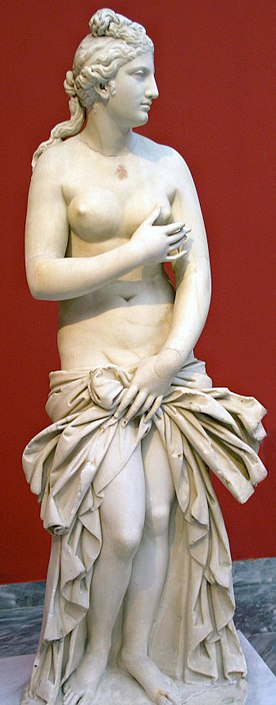
\includegraphics[width=0.7\textwidth,keepaspectratio]{pictures/NAMA_Aphrodite_Syracuse.jpg}%
	\caption*{Aphrodite: Greek goddess of Love? Or scheming internet billionaire?}%
	\label{aphrodite}%
\end{figure}%

\section{Classical AI}

Is the people of Troy, championed by Hector. Helen is rightfully theirs, it was an Olympian stitch up from the outset. Aphrodite gave her to Paris, Hector’s brother.

\section{Deep Learning Community}

Deep learning is the horse that the Greeks cleverly fill with their heroes and wait for it to be taken inside the gates of Troy. Naively welcomed by the people of Troy as they believe it to be an omen of the durability of the city. In practice the Greeks run out and start slaughtering everyone.

\section{Symbolic Logic}

Symbolic logic is Paris. Good looking fellow who was promised the hand of Helen before he’d even met her. The deal was done in exchange for an apple. Not particularly effective in battle, but gets off quite a lucky shot at some point. Is easily defeated by Menelaus in a one on one fight. Eventually killed by Philoctetes’s bow.

\section{Google}

Google as Menelaus, the husband of Helen. The marriage between Helen and Menelaus was what triggered all the attention in the first place. Everyone in Greek society wanted her, but after much deliberation and debate she was betrothed to Menelaus. To prevent trouble, the Greeks agreed a pact among themselves to defend the marriage. Unknown to Menelaus though, Helen had already been given to Paris by Aphrodite some time before (who had swapped her for an apple).

\section{Microsoft}

Microsoft as Agamemnon, the elder statesmen of the Greeks, perhaps not as in touch with modern Greek thinking as some others, but he commands enormous respect and still has many qualities. Some family history with the gods which complicates things for him.

\section{Facebook}

Facebook as Odysseus. He hid away when the initial call to arms was made, but once he realized the inevitability of the battle he joined in with vigor. Fundamentally he doesn't care so much about Helen. Cunning. Keen on his wife Penelope, who’s back in Ithaca. There’s also more story to come from this one.

\section{Apple}

Apple as Achilles, good looking, very fine hardware, and favored by the gods. However, he’s spent a large part of the battle so far sulking in his tent (he has a history with Agamemnon), may well be stirred to emerge at a critical moment to try and claim the plaudits.

\section{Amazon}

Amazon as Philoctetes, left behind early on because he had a smelly foot, but turns up late on to play a critical role when everyone realises that he’s the one with access to the hardware they need to kill Paris.

\section{``Deep Learning Conspiracy''}

The “deep learning conspiracy” is Cassandra. Cassandra told the truth but people were doomed not to believe her. In a special twist for our story, Cassandra gets a big one right, and after that everyone believes everything she says.

\section{OpenAI}

Neoptolemus (literally ``New Warrior'') is OpenAI. Turns up at the end, is very young, a teenager at most. Favored by the gods because of his progeny. His nature is unclear, depending on what source you read he is either depicted as brutal or kindly.

\section{Baidu}

Baidu as Aeneas, the Greek ideas of freedom and democracy are all very well, but there’s nothing quite like well organized empire for dominating the Mediterranean. Aeneas was a Trojan minor hero who went off to found the city of Rome.

\section{IBM}

IBM as Hercules, did some really good work in the past, including carrying the heavens on shoulders, killing some bothersome beasts and a lot of stable cleaning. Held in great respect by all the current combatants, but he’s not actually present at Troy. In a nice twist though, he will turn up again later in spirit form, along with Agamemnon, to give some advice to Odysseus.

\section{The Wider Greek World}

While the Trojan wars are widely written about, and even studied at schools, the story focuses on a group of misogynistic men, with fragile egos who, fall out over perceived slights and are chasing seductive goals of little true worth.

Meanwhile, back in wider Greek society, who knows what Pythagorous is up to? The aspects of the Greeks we value today: democracy, science and mathematics, get very little mention in their tales of heroes. While a battle raged around Troy, one wonders if the real story was what all the more sensible Greeks were getting up to. Maybe the wider Greek world is those people in machine learning and related communities who are simply driving forward with tangible useful goals on elegant problems of practical interest, just like we always did before our heads were all turned by Helen.

\chapter{The Future of AI Meeting}

On 15th September, 1830, the Liverpool and Manchester Railway opened. It was the first passenger railway. It is said that when rail travel was first proposed fears were voiced that travel at high speeds would cause asphyxia or permanently damage passengers’ eyes. Heady speeds of 50 km/h were unheard of at the time.

The first death on the railways actually occurred the day they opened. The MP for Liverpool disembarked from a stationary train and, in an attempt to greet the Duke of Wellington, he was run over by George Stephenson’s Rocket. His eyes and breathing had survived the initial journey just fine, but his legs were parted from his body under the Rocket’s wheels and he died later in a local hospital. Nowadays, we know not to disembark unless the train’s in a station.

The challenge of predicting the consequences of new technology is non trivial but the debate over what our AI futures holds sometimes has the feeling that we are predicting death by asphyxia or blindness, each induced by rapid motion.

A recent resurgence in popular fears about AI was triggered by Elon Musk, investor in DeepMind, who warned that humanity was ‘summoning the demon’. The previous chapter in this series parodied events in the field as a Homeric Greek tragi-comedy, in this chapter I’ll try and give some perspective on the evolving futures debate.

Ancient Greeks (featured in the last chapter in this series) weren't just famous for Homeric legend. They were also famous for politics and philosophy. Our idea of philosophy comes from Plato’s description of Socrates, the man who talked all thoughts and ideas through. He didn't believe in the written word, he believed in discussion and persuasion.

Understanding and validating the predictions of others requires that we first actually listen to what they are saying, the next challenge is in unpicking what their words actually mean. The recent debate about AI is occurring across different academic boundaries because the effects are expected to be so widespread.

Understanding people across different academic boundaries is particularly difficult. Firstly because, as academics, we are often more fond of talking than listening, but secondly because in each of our subfields there is a Babel-like propagation of terminology: each word means a different thing to each of us. Ethics, models, morals, noise, generalisation, mechanisms even probability. There are many barriers to communication, and Google translate will not do the job for us. Overcoming them requires patience and understanding.

I do believe we are participating in some form of revolution, but it has been ongoing for 300 years going back to Thomas Newcomen’s steam engine. In terms of the emergence of machine learning as a widespread technology and its effect on AI we won’t know its particular significance until the narratives are written well into our futures.

However, many of the ideas that are being debated are extremely important, both for researchers and the public. But the reaction of the machine learning community, including myself, sometimes varies between incredulity and ridicule. To move forward we need to change that reaction to accepting and our response to educating. Both ourselves and others. We need to take very seriously the way we are perceived and what our impact on the society around us is.

In response to the increased interest NIPS 2015 hosted a Symposium on Machine Learning in Society. A few weeks later, in January, the NYU Centre for Data Science recently convened a meeting to bring experts together, not just the worriers, but developers of AI systems, economists, futurologists, philosophers, psychologists, roboticists. 

\section{Future of AI meeting at NYU}

The remit of the “Future of AI” was to be cross-disciplinary covering the potential and pitfalls of our AI solutions. It was split into two parts, the first day was public and focused more on the potential of AI. We heard leading academics talk, and speakers from companies such as Google, Facebook, Microsoft, Mobileye and Nvidia each told of how core it is to their strategy. The roster of corporate speakers was also impressive, each company was represented typically by a CEO or a CTO.

Some speakers talked grandly of the ability of AI to solve challenges such as tackling climate, it was left to Thomas Dietterich, in one of the discussions, to point out that we aren’t going to solve climate by ‘deep learning’. That’s a key point to me, and one needs wider understanding. There’s nothing in the very recent developments in machine learning that significantly affects our ability to model and make predictions in complex systems where data is scarce. For climate change, our ability to access only one earth means that data is particularly scarce.

We heard Sebastian Seung speaking on the connectome: the mapping of the wiring of the human brain, and he also touched upon ‘uploading’, the idea that we could live virtually after our deaths by emulating ourselves on computers. I didn’t speak directly to Sebastian, but I think he has the right amount of skepticism about the viability of these ideas. However, I do worry that the credence he gives them is taken somewhat as a green light for rather fantastic (as in fantasy, not as in brilliant) ideas about where our immediate futures lie. I would agree that we are further down the technological road to ‘uploading’ than Tutankhamun’s high priests were when they liquefied his brain and sucked it out through his nose\footnote{A process known as excerebration, which is probably closer to us in the scale of required technological developments than the rather more delicate process of extracting the state of $10^14$ synapses via the nasal or any other passage.}, but not \textit{much} further.

Although the idea of uploading is a wonderful literary meme, such sensationalist perspectives can have the effect of overwhelming the more reasoned ideas we were hearing from attendees such as Bernhard Schölkopf who was emphasizing the importance of causal reasoning in intelligence.

\section{Chatham House Rule}

The second part of the meeting (days 2 and 3) the sessions were closed. They were at the same time more interdisciplinary but also more focused. They included economists, philosophers, psychologists, cognitive scientists and futurologists. The aim being to stimulate a wide ranging debate about our AI future and its effect on society.

Chatham House Rules mean that we can summarise the essence of what was said but not by whom, unless they gave their explicit permission. This rule is likely necessary because for an open debate on the pitfalls people need to be secure that their words won’t be sensationalized, particularly in the instances where they may have been playing devil’s advocate.

Speakers included very well known figures such as Erik Brynjolfsson (co-author with Andrew McAfee of “The Second Machine Age”), Nick Bostrom (author of “Superintelligence”) and Max Tegmark (founder of the “Future of Life” institute).

Hearing the economists’ discussion on productivity caused me to think a little more about the issue of jobs. I think I’m yet to be fully persuaded that anything dramatic is about to happen, my Dad’s job is different from mine and his was different from my grandfather’s. My grandmother worked full time at a time when it was unusual for women to do so, my wife does so when it is more common but she still experiences a working environment that has a structure designed by males and an environment dominated by males.

In the 1970s when \textit{they} were predicting the future, Xerox PARC postulated the idea of the paper free office. They developed the mouse and the graphical user interface. Nearly 50 years later, and there’s a pad of paper by my side as I write, and I just signed a paper check for my breakfast. Not only that, but paper consumption drastically increased in the 1980s and 1990s as a \textit{result} of the computer\footnote{Today that trend may have reversed due to widespread use of tablets, but as recently as 2012 the Economist was reporting on the widespread use of paper.}. Although thinking about the future did help: after all, regardless of the paper either side of me the mouse and the GUI did come into being.

However, by analogy, it might be that in the near term artificial intelligence won’t eliminate the need for the intellectual labor force, but actually (initially) increase it. Future prediction is fraught with uncertainty. We should be very wary of precise narratives that make strong claims.

There was a wide range of talks, other speakers covered areas such as the law, value systems and cognitive robotics (in particular our desire to embody intelligence).

\section{Perspective}

Events like the ``Future of AI'' are vital for extending the debate, achieving a shared set of objectives. However, it can be problematic when particular aspects aren't covered.

One particular facet of debates on AI is they assume some kind of mystical quality. In particular, we seem to all think of ourselves and our intelligence as something very special, holy even, the ghost in the machine. But with our self-idolization comes a Icarian fear of what it might mean to emulate those characteristics that we perceive of as uniquely human.

The recent advances in AI are all underpinned by machine learning. Machine learning is data driven and connects closely to statistics. This means that there is a smooth continuum between statistics on the one end, machine learning in the middle and ``artificial intelligence'' at the far end. The recent developments in AI are entirely underpinned by data. But data was almost never mentioned in the meeting.

This seems to me part of dangerous (and fairly pervasive) tendency to separate our discussion on AI from our discussion on data. Machine learning is not just the principle technology underpinning the recent success stories in AI, it is, along with statistics, the principle technology driving our agenda in data science. This is particularly interesting because the NYU meeting was hosted by the NYU Centre for Data Science, so it is not as if attendees were unaware of this (Yann Le Cun, one of the main conveners of the meeting is most certainly extremely aware of this).

Perhaps another explanation for the apparent absence of data\footnote{I mean the absence of data as a subject. Of course there was an absence of data to validate arguments too, but that’s somewhat inevitable when there’s an amount of future-prediction going on.} is that there was a necessary interest in framing the discussion through the wider public debate. Two particular ideas seem to capture the public imagination. In the near term people are worried about loosing their jobs to “robots”, in the further term people are worried about loosing ``humanity’s earthly inheritance'' to the robots. They are worried about killer terminator robots.

With this in mind, the last session in New York was on “AI Safety”. Quite an emotive term itself (we don’t normally worry about safety for things that aren't dangerous). There were a range of interesting talks including Stuart Russell and Michael Littman. We also heard from Nick Bostrom whose book “Superintelligence” conceived future potential responses to AI, more of that in the next episode in this series.

On return to the UK, I went straight to the Royal Society in London to participate in evidence gathering for the Royal Society’s working group on Machine Learning. Our remit is focused on the next five to ten years, and data is featuring very prominently in our discussions. The sessions themselves could not have been more contrasting. Small group evidence gathering, with particular questions targeted at invited experts who had responded to an earlier call for written evidence.

There will be a report arising from the Royal Society Working Group that I should not prejudge. However, it did feel rather extraordinary to go (in a single 24 hour period) from chatting (briefly) to Daniel Kahneman to interviewing Baroness O’Neill. I was also relieved at the extent to which the Royal Society working group acknowledges the importance of data in the debate.

Having said that it’s important to emphasize that both approaches: the small focused meeting of the Royal Society, and the larger, interdisciplinary debate of the Future of AI meeting, are a vital part of informing and understanding how our new technologies may effect us.

I’m looking forward to more in this space.

\chapter{The Singularians}

Religious belief offers the promising and delightful idea of an eternal life in paradise. But as a non believer one of the things you need come to terms with is the finality of death\footnote{There may be many reasons why people choose to be non religious. I once joined the UK’s British Humanist Association, but I found the preaching nature of the literature they sent in my welcome pack somewhat disturbing, so despite being broadly aligned with their perspective, I felt alienated by their pious narrative. This may make me a contrarian, and perhaps this chapter should be read in that light.}. There is a happy side effect of realising that since death is final, you realize the importance of extracting value from your limited life: technically this is known as a ‘finite horizon effect’\footnote{The average American experiences over an hour a day on TV adverts. Of course this is only an average, imagine what a really good American could manage.}.

\begin{figure}[htbp]%
	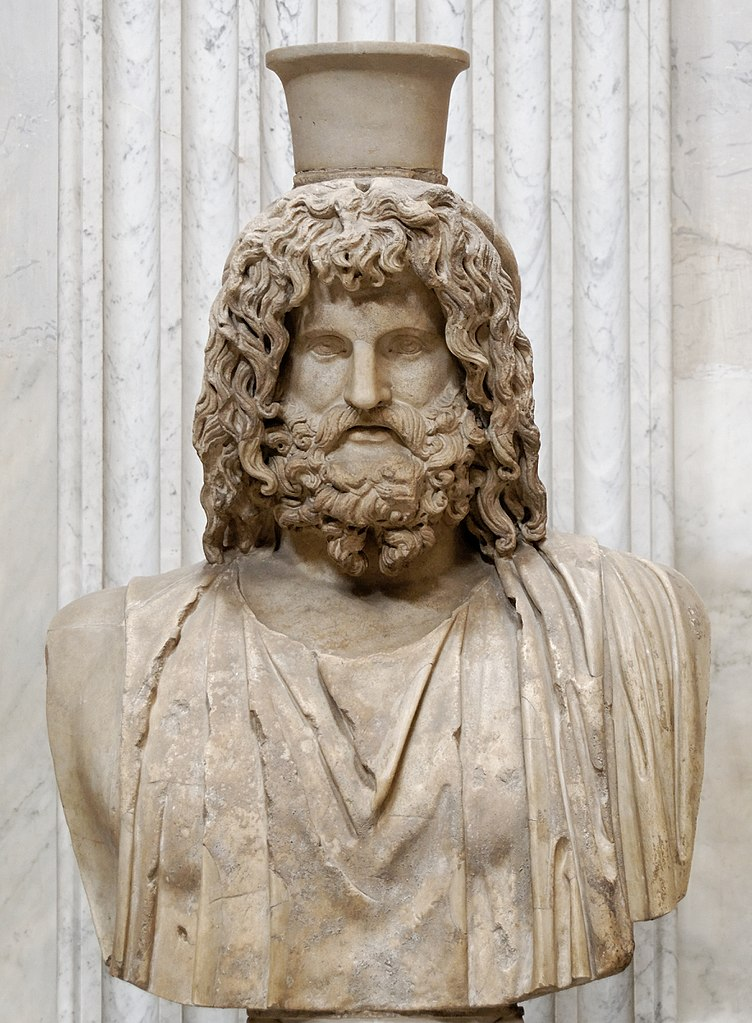
\includegraphics[width=\textwidth]{pictures/Serapis_Pio-Clementino.jpg}%
	\caption*{Greek gods have beards and live on a mountain.}%
	\label{greek-gods}%
\end{figure}%

However, I’m beginning to suspect that not everyone of irreligious persuasion is quite as comfortable with this realisation. Recent breakthroughs in machine learning are triggering emerging debates that, at first, I found difficult to interpret. But through some reading, some thought and some conversation with colleagues, I believe there’s a plausible latent cause for these discussions. Everything becomes much clearer if you posit that in many influential minds there’s an emerging strand of belief, of faith, that I’ve come to think of as “Singularism”\footnote{Some post-writing research (always the best kind) showed this movement is also called Transhumanism or Singularitarianism. But the first sounds a little bit like people who believe they are animals born in human bodies, and the second is difficult to say (imagine when there’s a someone who wants to sever links between Singularitarianists and the state, they will have to say they are a singularitariodisestablishmentarian).}.

\section{The Day of Judgment: Technological Singularity}

The prophets of Singularism foretold that there would come a time when the rate of progress of technology accelerated so much that it outpaced human ability to keep up. To a Singularian this time is nigh.

Singularism is to religion what scientology is to science. Scientology is religion expressing itself as science and Singularism is science expressing itself as religion.

Religion historically had a seat at the table of power. Either as host or guest of honour. Close interaction between power and priesthood. Those that promise the technological singularity also hold high office. They are embedded in leading companies and even some of our top universities.

We each should be free to hold our own beliefs, and having faith in the singularity should also be seen of as a belief. However, one way religion can impinge on society is if people become so enamored of its teachings that they fail to fulfill their practical everyday duties, the functions of life or leadership. It is a problem when life becomes a prelude to afterlife. Obsession with the technological singularity may be beginning to have that effect.

\subsection{The Consequence}

There are very real challenges facing the machine learning community, very real opportunities, but a lot of the popular literature fails to address these challenges and instead presents narratives that appeal to each of the religious facets of Singularism.

Some of the appeal of this literature might originate in a kind of technopop philosophy: framing popular ideas in technical language so as to provide a flavour of plausibility. Although sometimes technopop feels inaccurate, some books take on a more arcane turn, more in keeping with religious texts. To the uninitiated the concepts may appear powerful and intimidating, but an alternative interpretation of them is rather more of mundane misunderstandings followed by overly convolved consequences.

I’m a great believer in society’s sustenance of different individual beliefs and philosophies. A robust variation of approaches to life seems, perhaps, the only safety net we have against the uncertainties we experience each day and across our lives. But when a set of faith-based arguments begins to persuasively influence the wider debate in a (potentially) damaging manner, then I think this needs highlighting.

The damage being caused by the Singularians is arising from their apparent authority, yet their failure to address significant challenges. Much of the debate around the long term future of AI omits many of the real challenges that we face right now, and concerns itself with hand-wringing about the singularity as the day of judgment and the process by which the chosen will be anointed.

As a micro-exemplar of this recently we can look at the UK Artificial Intelligence company DeepMind. Their launch onto the public consciousness after their purchase by Google was accompanied by a wave of propheteering about the imminent dooms of AI. But in practice, their first (minor) misstep has taken place over their failure to be more open about agreements with the Royal Free hospital concerning 1.6 million patients worth of data\footnote{DeepMind’s purchase by Google was the trigger for Elon Musk to warn that we were ‘releasing the demon’ of artificial intelligence. As an investor in DeepMind Musk was persuaded by their technologies. That human intelligence through artificial systems was nearby. However, as a non-expert in AI he was unable to appreciate the myriad ways in which we are far from that goal. Even the extremely impressive achievement of AlphaGo is long distant from human intelligence. It is domain-focussed and data-inefficient. In the meantime DeepMind have, perhaps at the behest of clinicians from the Royal Free Hospital, set up a health division. In a domain in which they had no track record, a group of clinicians thought it appropriate to engage DeepMind on 1.6 million patientsworth of data, without consulting those patients. The scale of the deal only emerged through a piece in the New Scientist. Knowing colleagues at DeepMind, I would declare them not guilty on both counts. I do not believe they are close to resolving the mechanisms by which human intelligence operates (although they are a world leading lab in this area, with some magnificent achievements to their name). And they are entering the health arena with the best of intentions. But in the real world, the best of intentions is often not enough. There are major issues with an individual’s control of their personal private data. And the fact that a company and group of clinicians, through naivety, can be blind to these issues despite their regular presence in the media does not bode well.}.

Data-sharing is among the great many challenges associated with the rising influence of algorithmic decision making on our lives, but there is little to no mention of data in much of the debate around AI, nor is there a realization that individual privacy is the keystone of our protection against the rise of the algorithm. The present danger is not that we create an artificial general intelligence to dominate our lives, but that a rather more mundane algorithms we distribute today will increasingly restrict our existing freedoms.

But why worry about surly earthly bonds when heaven’s saintly kiss is apparently within reach? The focus of much of the AI debate seems entirely on how to avoid the pitfalls of the perceived paradise. Singularism has its day of judgment, “the singularity”. For intelligence this is the day where we create intelligent machines which themselves have the ability to create new intelligent machines. The resulting cascade affect brings about runaway intelligence.

Like many religions, Singularism acknowledges two possible outcomes from the day of judgment, the singularity. Superintelligence focuses on ensuring that our heaven, our galactic inheritance (e.g. immortal life via ‘brain uploading’), is achieved at the expense of hell (death by killer terminator robot).

\subsection{Intelligent Overlords}

Also inherent in this new religion is the idea of artificially intelligent overlords, either beneficent or malevolent (the final nature of the new religion is not yet clear).

Although stimulating for societal debate, the challenges of the high church of Singularism are deflecting us from the humdrum of the actual decisions we need to make. It is through data that our intelligent systems are built, but it seems that we are not communicating the actualities of today’s technology and we are encouraging images of an intelligent future that are little removed from ideas people proposed half a century ago.



\chapter{Discussion of 'Superintelligence:\\Paths, Dangers, Strategies'}

\begin{marginfigure}%
    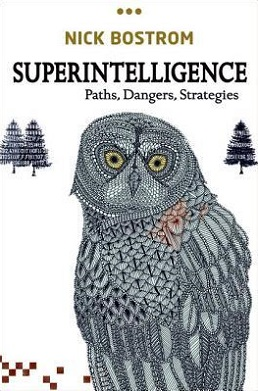
\includegraphics[width=\marginparwidth]{pictures/Superintelligence.jpg}%
    \caption*{Cover of Superintelligence.}
    \label{superintelligence}%
\end{marginfigure}%

This chapter is a discussion of Nick Bostrom’s book “Superintelligence”. The book has had an effect on the thinking of many of the world’s thought leaders. Not just in artificial intelligence, but in a range of different domains (politicians, physicists, business leaders). In that light, and given this series is about the ``Future of AI'', it seemed important to read the book and discuss his ideas.

In an ideal world, this chapter would certainly have contained more summaries of the books arguments and perhaps a later update will improve on that aspect. For the moment the review focuses on counter-arguments and perceived omissions (the chapter already got too long with just covering those).

Bostrom considers various routes we have to forming intelligent machines and what the possible outcomes might be from developing such technologies. He is a professor of philosophy but has an impressive array of background degrees in areas such as mathematics, logic, philosophy and computational neuroscience.

So let’s start at the beginning and put the book in context by trying to understand what is meant by the term “superintelligence”.

\section{Defining Intelligence}

In common with many contributions to the debate on artificial intelligence, Bostrom never defines what he means by intelligence. Obviously, this can be problematic. On the other hand, superintelligence is defined as outperforming humans in every intelligent capability that they express.

Personally, I have developed the following definition of intelligence: “Use of information to take decisions which save energy in pursuit of a given task”\footnote{Think of this as a pocketknife definition of intelligence. It’s designed to be portable and fulfill a variety of roles (it even has a bit for intelligent removal of stones from horses hooves).}. Here by information I might mean data or facts or rules, and by saving energy I mean saving ‘free’ energy\footnote{Heat engines are systems for converting heat into useful work. By my definition intelligence is conducted through an \textit{inference engine} that is for taking information and using it to conserve work (by avoiding things we didn't need to do).}.

However, accepting Bostrom’s lack of definition of intelligence (and perhaps taking note of my own), we can still consider the routes to superintelligence Bostrom proposes. It is important to bear in mind that Bostrom is worried about the effect of intelligence on 30 year (and greater) timescales. These are timescales which are difficult to predict over. I think it is admirable that Nick is trying to address this, but I’m also keen to ensure that particular ideas which are at best implausible, but at worst a misrepresentation of current research, don’t become memes in the very important debate on the future of machine intelligence.

\section{Technological Singularities}

A technological singularity is when a technology becomes ‘transhuman’ in its possibilities, moving beyond our own capabilities through self improvement. It’s a simple idea, and often there’s nothing to be afraid of. For example, in mechanical engineering, we long ago began to make tools that could manufacture other tools. And indeed, the precision of the manufactured tools outperformed those that we could make by hand. This led to a ‘technological singularity’ of precision made tools. We developed ‘transhuman’ milling machines and lathes. We developed ‘superprecision’, precision that is beyond the capabilities of any human. Of course there are physical limits on how far this particular technological singularity has taken us. We cannot achieve infinitely precise machining tolerances.

In machining, the concept of ‘precision’\footnote{Not machine precision, but machining precision.} can be defined in terms of the ‘tolerance’ that the resulting parts are made to. Unfortunately, the lack of a definition of intelligence in Bostrom’s book makes it harder to ground the argument. In practice this means that the book often exploits different facets of intelligence and combines them in worse case scenarios while simultaneously conflating conflicting principles.

\section{Embodied Intelligence}

The book gives little thought to the differing natures of machine and human intelligence. For example, there is no acknowledgment of the embodied nature of our intelligence\footnote{Current machine intelligence is very different from human intelligence because it is disembodied. In particular, the rate at which computers can talk to each other far exceeds that with which humans can interact. That is what makes our intelligence special. I have referred to it as ‘locked in’ intelligence in a previous chapter. Bostrom doesn't seem to acknowledge this. He talks about collective emulation of brains as one potential future and segues between embodied and disembodied intelligences opportunistically as the argument requires.}. There are physical constraints on communication rates. For humans these constraints are much stronger than for machines. Machine intelligences communicate with one another in gigabits per second. Humans in bits per second. For our relative computational abilities the best estimates are that, in terms of underlying computation in the brain, we are computing much quicker than machines. This means humans have a very high compute/communicate ratio. We might think of that as an \textit{embodiment factor}. We can compute far more than we can communicate, leading to a backlog of conclusions within our own minds\footnote{If this were not true then we could perhaps more easily upload our brains, making the Singularians very happy.}. Much of our human intelligence seems doomed to remain within ourselves. This dominates the nature of human intelligence. In contrast, this phenomenon is only weakly observed in computers, if at all. Computers can distribute the results of their intelligence at approximately the same rate that they compute them.

Bostrom’s idea of superintelligence is an intelligence that outperforms us in all its facets. But if our emotional intelligence is a result of our limited communication ability, then it might be impossible to emulate it without also implementing the limited communication. Since communication also affects other facets of our intelligence we can see how it may, therefore, be impossible to dominate human abilities in the manner which the concept of superintelligence envisages. A better definition of intelligence would have helped resolve these arguments.

My own belief is that we became individually intelligent through a need to model each other (and ourselves) to perform better planning\footnote{Modelling in the sense of predictive modelling. It may be to understand intent and depending on context, or to determine our individual collaborative or competitive response. When planning into the future that also requires a model for ourselves and how we are likely to respond to given circumstances. This model might be a candidate for our perceived sense of self.}. So we evolved to undertake collaborative planning and developed complex social interactions. As a result our species, our collective intelligence, became increasingly complex (on evolutionary timescales) as we evolved greater intelligence within each of the individuals that made up our social group. Because of this process I find it difficult to fully separate our collective intelligence from our individual intelligences. I don’t think Bostrom suffers with this dichotomy because my impression is that his book only views human intelligence as an individual characteristic. My feeling is that this is limiting because any algorithmics we create to emulate our intelligence will actually operate on societal scales and the interaction of the artificial intelligence with our own should be considered in that context\footnote{As a result the debate transcends technology, philosophy, psychology and social science.}.

\section{Prediction, Uncertainty and Intelligence Saturation}

As humans, we are a complex society of interacting intelligences. Any predictions we make within that society would seem particularly fraught. Intelligent decision making relies on such predictions to quantify the value of a particular decision (in terms of the energy it might save). But when we want to consider future plausible scenarios we are faced with exponential growth of complexity in an already extremely complex system.

In practice we can make progress with our predictions by compressing the complex world into abstractions: simplifications of the world around that are sufficiently predictive for our purposes, but retain tractability. However, using such abstractions involves introducing \textit{model uncertainty}. Model uncertainty reflects the unknown way in which the actual world will differ from our simplifications.

Practitioners who have performed sensitivity analysis on time series prediction will know how quickly uncertainty accumulates as you try to look forward in time. There is normally a time frame ahead of which things become too misty to compute any more. Further computational power doesn't help you in this instance, because uncertainty dominates. Reducing model uncertainty requires exponentially greater computation\footnote{In practice this means that our choice of model abstraction depends on the timescales over which we wish to compute, for example we use different models for our climate predictions versus our weather predictions despite the underlying physical system being the same.}. We might try to handle this uncertainty by quantifying it, but even this can prove intractable.

So just like the elusive concept of infinite precision in mechanical machining, there is likely a limit on the degree to which an entity can be intelligent. We cannot predict with infinite precision and this will render our predictions useless on some particular time horizon.

The limit on predictive precision is imposed by the exponential growth in complexity of exact simulation, coupled with the accumulation of error associated with the necessary abstraction of our predictive models. As we predict forward these uncertainties can saturate dominating our predictions. As a result we often only have a very vague notion of what is to come. This limit on our predictive ability places a fundamental limit on our ability to make intelligent decisions.

There was a time when people believed in perpetual motion machines (and quite a lot of effort was put into building them). Physical limitations of such machines were only understood in the late $19^{th}$ century (for example the limit on efficiency of heat engines was theoretically formulated by Carnot). We don’t yet know the theoretical limits of intelligence, but the intellectual gymnastics of some of the entities described in Superintelligence will likely be curtailed by the underlying mathematics\footnote{Singularities are normally unsustainable in practice because the mechanisms which they exploit at launch are normally exhausted and saturation occurs. There may be an exponential explosion but if it encounters problems of exponential complexity the irresistible force encounters the immovable object and a stalemate (or saturation) results.}. In practice the singularity will saturate, it’s just a question of where that saturation will occur relative to our current intelligence. Bostrom thinks it will be a long way ahead, I tend to agree but I don’t think that the results will be as unimaginable as is made out. Machines are already a long way ahead of us in many areas (weather prediction for example) but I don’t find that unimaginable either.

Unfortunately, in his own analysis, Bostrom hardly makes any use of uncertainty when envisaging future intelligences. In practice correct handling of uncertainty is critical in intelligent systems. By ignoring it Bostrom can give the impression that a superintelligence would act with unerving confidence. Indeed the only point where I recollect the mention of uncertainty is when it is used to unnerve us further. Bostrom refers to how he thinks a sensible Bayesian agent would respond to being given a particular goal. Bostrom suggests that due to uncertainty it would believe it might not have achieved its goal and continue to consume world resource in an effort to do so. In this respect the agent appears to be taking the inverse action of that suggested by the Greek skeptic Aenesidemus, who advocated suspension of judgment, or epoché, in the presence of uncertainty. Suspension of judgment (delay of decision making) meaning specifically ‘refrain from action’. That is indeed the intelligent reaction to uncertainty. Don’t needlessly expend energy when the outcome is uncertain (to do so would contradict my definition of intelligent behavior). This idea emerges as optimal behavior from a mathematical treatment of such systems when uncertainty is incorporated.

This meme occurs through out the book. The ``savant idiot''\footnote{An ``idiot savant'' is a person with limited intelligence who has a particular gift (insight or memory etc). It therefore seems appropriate to define “savant idiot” to indicate the idea of a “superintelligence” that does particularly stupid things. Not sure of the correctness in the French here, google translate offers “génie fou” as an alternative.}, a gifted intelligence that does a particular thing really stupidly. As such it contradicts the concept of superintelligence. The superintelligence is better in all ways than us, but then somehow must also be taught values and morals. Values and morals are part of our complex emergent human behaviour. Part of both our innate and our developed intelligence, both individually and collectively as a species. They are part of our natural conservatism that constrains extreme behavior. Constraints on extreme behaviour are necessary because of the general futility of absolute prediction. Just as in machining, we cannot achieve infinitely precise prediction.

Another way the savant idiot expresses itself in the book is through extreme confidence about its predictions in the future. The premise is that it will agressively follow a strategy (potentially to the severe detriment of humankind) in an effort to fulfill a defined ‘final goal’. We’ll address the mistaken idea of a simplistic final goal below.

With a shallow reading Bostrom’s ideas seem to provide an interesting narrative. In the manner of an Ian Fleming novel, the narrative is littered with technical detail to increase the plausibility for the reader.16 However, in the same way that so many of Blofeld’s\footnote{Bond’s nemesis and head of the organization SPECTRE.} schemes are quite fragile when exposed to deeper analysis, many of Bostrom’s ideas are as well.

In reality, challenges associated with abstracting the world render the future inherently unpredictable, both to humans and to our computers. Even when many aspects of a system are broadly understood (such as our weather) prediction far into the future is untenable due to propagation of uncertainty through the system. Uncertainty tends to inflate as time passes rendering only near term prediction plausible. Inherent to any intelligent behavior is an understanding of the limits of prediction. Intelligent behaviour withdraws, when appropriate, to the ``suspension of judgement'', inactivity, the epoché. This simple idea finesses many of the challenges of artificial intelligence that Bostrom identifies.

\section{Whole Brain Emulation}

Large sections of the book are dedicated to whole brain emulation, under the premise that this might be achievable before we have understood intelligence (superintelligence could then achieved by hitting the turbo button and running those brains faster). Simultaneously, hybrid brain-machine systems are rejected as a route forward due to the perceived difficulty of developing such interfaces.

Such unevenhanded treatment of future possible paths to AI makes the book a very frustrating read. If we had the level of understanding we need to fully emulate the brain, then we would know what is important to emulate in the brain to recreate intelligence. The path to that achievement would also involve improvements of our ability to directly interface with the brain. Given that there are immediate applications with patients, e.g. with spinal problems or suffering from ALS, I think we will have developed hybrid systems that interface directly with the brain a long time before we have managed a full emulation of the human brain. Indeed, such applications may prove to be critical to developing our understanding of how the brain implements intelligence.

Perhaps Bostrom’s naive premise about the ease of brain emulation comes form a lack of understanding of what it would involve. It could not involve an exact simulation of each neuron in the brain down to the quantum level (and if it did, it would be many orders of magnitude more computationally demanding than is suggested in the text). Instead it would involve some level of abstraction. Abstraction as to those aspects of the biochemistry and physics of the brain that are important in generating our intelligence. Modelling and simulation of the brain would require that our simulations replace actual mechanism with those salient parts of those mechanisms that the brain makes use of for intelligence.

As we have mentioned in the context of uncertainty, an understanding of this sort of abstraction is missing from Superintelligence, but it is vital in modelling, and, I believe, it is vital in intelligence. Such abstractions require a deep understanding of how the brain is working, and such understandings are exactly what Bostrom says are impossible to determine for developing hybrid systems.

Over the 30 year time horizons that Bostrom is interested in, hybrid human-machine systems could become very important. They are highly likely to arise before a full understanding of the brain is developed, and if they did then they would change the way society would evolve. That’s not to say that we won’t experience societal challenges, but they are likely to be very different from the threats that Bostrom perceives. Importantly, when considering humans and computers, the line of separation between the two may not be as distinctly drawn as Bostrom suggests. It wouldn’t be human vs computer, but augmented human vs computer\footnote{For example, can a human working in collaboration with a computer beat the best pure computer players at Go or Chess?}.

\section{Dedication of Resources and Control of Progress}

One aspect that, it seems, must be hard to understand if you’re not an active researcher is nature of technological advance at the cutting edge. The impression Bostrom gives is that research in AI is all a set of journeys with predefined goals. It’s therefore merely a matter of assigning resources, planning, and navigating your way there. In his strategies for reacting to the potential dangers of AI, Bostrom suggests different areas in which we should focus our advances (which of these expeditions should we fund, and which should we impede). In reality, we cannot switch on and off research directions in such a simplistic manner. Most research in AI is less of an organized journey, but more of an exploration of uncharted terrain. You set sail from Spain with government backing and a vague notion of a shortcut to the spice trade of Asia, but instead you stumble on an unknown continent of gold-ridden cities. Even then you don’t realize the truth of what you discovered within your own lifetime\footnote{Columbus went to his grave not realizing that the land he’d discovered was formerly unknown to Europeans. He still thought he’d reached Asia.}.

Even for the technologies that are within our reach, when we look to the past, we see that people were normally overly optimistic about how rapidly new advances could be deployed and assimilated by society. In the 1970s Xerox PARC focused on the idea that the ‘office of the future’ would be paperless. It was a sensible projection, but before it came about (indeed it’s not quite here yet) there was an enormous proliferation of the use of paper, so the demand for paper increased.

Rather than the sudden arrival of the singleton, I suspect we’ll experience something very similar to our ‘journey to the paperless office’ with artificial intelligence technologies. As we develop AI further, we will likely require more sophistication from humans. For example, we won’t be able to replace doctors immediately, first we will need doctors who have a more sophisticated understanding of data. They’ll need to interpret the results of, e.g., high resolution genetic testing. They’ll need to assimilate that understanding with their other knowledge. The hybrid human-machine nature of the emergence of artificial intelligence is given only sparse treatment by Bostrom. Perhaps because the narrative of such co-evolution is much more difficult to describe than an independent evolution.

The explorative nature of research adds to the uncertainties about where we’ll be at any given time. Bostrom talks about how to control and guide our research in AI, but the inherent uncertainties require much more sophisticated thinking about control than Bostrom offers. In a stochastic system, a controller needs to be more intelligent and more reactive. The right action depends crucially on the time horizon. These horizons are unknown. Of course, that does not mean the research should be totally unregulated, but it means that those that suggest regulation need to be much closer to the nature of research and its capabilities. They need to work in collaboration with the community.

Arguments for large amounts of preparatory work for regulation are also undermined by the imprecision with which we can predict the nature of what will arrive and when it will come. In 1865 Jules Verne\footnote{``From the Earth to the Moon'' by Jules Verne. A classic book. I particularly enjoyed the fact that they took some chickens with them, which, given the understanding at the time, seems very sensible and practical.} correctly envisaged that one day humans would reach the moon. However, the manner in which they reached the moon in his book proved very different from how we arrived in reality. Verne’s idea was that we’d do it using a very big gun. A good idea, but not correct. Verne was, however, correct that the Americans would get there first. One hundred and four years after he wrote the goal was achieved through rocket power (and without any chickens inside the capsule).

This is not to say that we shouldn’t be concerned about the paths we are taking. There are many issues that the increasing use of algorithmic decision making raises and they need to be addressed. It is to say that the nature of the concerns that Bostrom raises are implausible because of the imprecision of our predictions over such time frames.

\section{Final Goals and AI}

Some of Bostrom’s perspectives may also come from a lack of experience in deploying systems in practice. The book focuses a great deal on the programmed ‘final goal’ of our artificial intelligences. It is true that most machine learning systems have objective functions, but an objective function doesn’t really map very nicely to the idea of a ‘final goal’ for an intelligent system. The objective functions we normally develop are really only effective for simplistic tasks, such as classification or regression. Perhaps the more complex notion of a reward in reinforcement learning is closer, but even then the reward tends to be task specific.

Arguably, if the system does have a simplistic ‘final goal’, then it is already failing its test of superintelligence, even the simplest human is a robust combination of, sometimes conflicting, goals that reflect the uncertainties around us. So if we are goal driven in our intelligence, then it is by sophisticated goals (akin to multi-objective optimisation) and each of us weights those goals according to sets of values that we each evolve, both across generations and within generations. We are sophisticated about our goals, rather than simplistic, because our environment itself is evolving, implying that our ways of behaviour need to evolve as well. Any AI with a simplistic final goal would fail the test of being a ‘dominant intelligence’. It would not be a superintelligence because it would under-perform humans in one or more critical aspects.

\section{Data and the Reality of Current Intelligence}

One of the routes explored by Bostrom to superintelligence involves speeding up implementations of our own intelligence. Such speed would not necessarily bring about significant advances in all domains of intelligence, due to fundamental limits on predictability. Linear improvements\footnote{Of course Moore’s law has meant that our improvements in speed have been super-linear (exponential) so far, but eventually the limits of computation will be reached. Even then it still took us around 20 years to go from beating humans at Chess to beating humans at Go, largely because, while both games are exponentially complex, Go has a much larger branching factor (about 10 times as big) and that factor appears in the exponent of the complexity, causing the complexity to increase dramatically.} in speed cannot deal with exponential increases in computational tractability. But Bostrom also seems to assume that speeding up intelligences will necessarily take them beyond our comprehension or control. Of course in practice there are many examples where this is not the case. IBM Watson’s won Jeopardy. But it did it by storing a lot more knowledge than we ever could, then it used some simplistic techniques from language processing to recover those facts: it was a fancy search engine. These systems outperform us, but they are by no means beyond our comprehension. Still, that does not mean we shouldn’t fear this phenomenon.

Given the quantity of data we are making available about our own behaviors and the rapid ability of computers to assimilate and intercommunicate, it is already conceivable that machines can predict our behavior better than we can. Not by superintelligence but by scaling up of simple systems. They have finessed the uncertainty by access to large quantities of data. These are the advances we should be wary of, yet they are not beyond our understanding. Such speeding up of compute and acquisition of large data is exactly what has led to the recent revolution in convolutional neural networks and recurrent neural networks. All our recent successes are just more compute and more data.

This brings me to another major omission of the book, and this one is ironic, because it is the fuel for the current breakthroughs in artificial intelligence. Those breakthroughs are driven by machine learning. And machine learning is driven by data. Very often our personal data. Machines do not need to exceed our capabilities in intelligence to have a highly significant social effect. They outperform us so greatly in their ability to process large volumes of data that they are able to second guess us without expressing any form of higher intelligence. This is not the future of AI, this is here today.

Deep neural networks of today are not performant because someone did something new and clever. Those methods did not work\footnote{By work here I mean outperform humans (or perform similarly to humans). They often worked in the other sense, but were displaced by methods that were as performant and easier to understand from a modelling perspective.} with the amount of data we had available in the 1990s. They work with the quantity of data we have now. They require a lot more data than any human uses to perform similar tasks. So already, the nature of the intelligence around us is data dominated. Any future advances will capitalise further on this phenomenon.

The data we have comes about because of rapid interconnectivity and high storage (this is connected to the low embodiment factor of the computer). It is the consequence of the successes of the past and it will feed the successes of the future. Because current AI breakthroughs are based on accumulation of personal data, there is opportunity to control its development by reformation of our rules on data.

Unfortunately, this most obvious route to our AI futures is not addressed at all in the book.

\section{Summary}

Debates about the future of AI and machine learning are very important for society. People need to be well informed so that they continue to retain their individual agency when making decisions about their lives.

I welcome the entry of philosophers to this debate, but I don’t think Superintelligence is contributing as positively as it could have done to the challenges we face. In its current form many of its arguments are distractingly irrelevant.

I am not an apologist for machine learning, or a promoter of an unthinking march to algorithmic dominance. I have my own fears about how these methods will effect our society, and those fears are immediate. Bostrom’s book has the feel of an argument for doomsday prepping. But a challenge for all doomsday preppers is the quandary of exactly which doomsday they are preparing for. Problematically, if we become distracted with those images of Armageddon, we are in danger of ignoring existent challenges that urgently need to be addressed.


\part{Building A Data Democracy}

Chapters in this part point out new questions we as a society need to answer to take good care of our data. Current regulations on data need to evolve, and the data landscape needs to be democratised, if we are to build a data democracy. But how can this be done?

To restore individual rights, and produce more of a sense of citizenship, we might consider the idea of a “data trust”: a mutual organisation formed to manage data on its members’ behalf. Data subjects would pool their data forming a trust, stipulating conditions under which data could be shared. The trust would retain a duty of care without conflicting goals such as making a profit or furthering a research career.

\chapter{Legislation for Personal Data:\\Magna Carta or Highway Code?}

Karl Popper is perhaps one of the most important thinkers from the 20th century. Not purely for his philosophy of science, but for giving a definitive answer to a common conundrum: ``Which comes first, the chicken or the egg?''. He says that they were simply preceded by an ‘earlier type of egg’. I take this to mean that the answer is neither: they actually co-evolved. What do I mean by co-evolved? Well broadly speaking there once were two primordial entities which weren't very chicken-like or egg-like at all, over time small changes occurred, supported by natural selection, rendering those entities unrecognisable from their origins into two of our most familiar foodstuffs of today.

I find the process of co-evolution remarkable, and to some extent unimaginable, or certainly it seems to me difficult to visualise the intermediate steps. Evolution occurs by natural selection: selection by the ‘environment’, but when we refer to co-evolution we are clarifying that this is a complex interaction. The primordial entities effect the environment around them, therefore changing the ‘rules of the game’ as far as survival is concerned. In such a convolved system certainties about the right action disappear very quickly.

What use are chickens and eggs when talking about personal data? Well, Popper used the question to illustrate a point about scientific endeavour. He was talking about science and reflecting on how scientific theories co-evolve with experiments. However, that’s not the point I’d like to make here. Co-evolution is very general, one area it arises is when technological advance changes society to such an extent that existing legislative frameworks become inappropriate. Tim Berners Lee has called for a Magna Carta for the digital age, and I think this is a worthy idea, but is it the right idea? A digital bill of rights may be the right idea in the longer run, but I don’t think we are ready to draft it yet. My own research is machine learning, the main technology underpinning the current AI revolution. A combination of machine learning, fast computers, and interconnected data means that the technological landscape is changing so fast that it is effecting society around us in ways that no one envisaged twenty years ago.

Even if we were to start with the primordial entities that presaged the chicken and the egg, and we knew all about the process of natural selection, could we have predicted or controlled the animal of the future that would emerge? We couldn't have done. The chicken exists today as the product of its environmental experience, an experience that was unique to it. The end point we see is one of is highly sensitive to very small perturbations that could have occurred at the beginning.

So should we be writing legislation today which ties down the behaviour of future generations? There is precedent for this from the past. Before the printing press was introduced, no one would have begrudged the monks’ right to laboriously transcribe the books of the day. Printing meant it was necessary to protect the ``copy rights'' of the originator of the material. No one could have envisaged that those copyright laws would also be used to protect software, or digital music. In the industrial revolution the legal mechanism of ‘letters patent’ evolved to protect creative insight. Patents became protection of intellectual property, ensuring that inventors’ ideas could be shared under license. These mechanisms also protect innovation in the digital world. In some jurisdictions they are now applied to software and even user interface designs. Of course even this legislation is stretched in the face of digital technology and may need to evolve, as it has done in the past.

The new legislative challenge is not in protecting what is innovative about people, but what is commonplace about them. The new value is in knowing the nature of people: predicting their needs and fulfilling them. This is the value of interconnection of personal data. It allows us to make predictions about an individual by comparing him or her to others. It is the mainstay of the modern internet economy: targeted advertising and recommendation systems. It underpins my own research ideas in personalisation of health treatments and early diagnosis of disease. But it leads to potential dangers, particularly where the uncontrolled storage and flow of an individual’s personal information is concerned. We are reaching the point where some studies are showing that computer prediction of our personality is more accurate than that of our friends and relatives. How long before an objective computer prediction of our personality can outperform our own subjective assessment of ourselves? Some argue those times are already upon us. It feels dangerous for such power to be wielded unregulated by a few powerful groups. So what is the answer? New legislation? But how should it come about?

In the long term, I think we need to develop a set of rules and legislation, that include principles that protect our digital rights. I think we need new models of ownership that allow us to control our private data. One idea that appeals to me is extending data protection legislation with the right not only to view data held about us, but to also ask for it to be deleted. However, I can envisage many practical problems with that idea, and these need to be resolved so we can also enjoy the benefits of these personalised predictions.

As wonderful as some of the principles in the Magna Carta are, I don’t think it provides a good model for the introduction of modern legislation. It was actually signed under duress: under a threat of violent revolution. The revolution was threatened by a landed gentry, although the consequences would have been felt by all. Revolutions don’t always end well. They occur because people can become deadlocked: they envisage different futures for themselves and there is no way to agree on a shared path to different end points. The Magna Carta was also a deal between the king and his barons. Those barons were asking for rights that they had no intention of extending within their fiefdoms. These two characteristics: redistribution of power amongst a powerful minority, with significant potential consequences for the a disenfranchised majority, make the Magna Carta, for me, a poor analogy for how we would like things to proceed.

The chicken and the egg remind us that the actual future will likely be more remarkable than any of us can currently imagine. Even if we all seek a particular version of the future this version of the future is unlikely to ever exist in the form that we imagine. Open, receptive and ongoing dialogue between the interested and informed parties is more likely to bring about a societal consensus. But can this happen in practice? Could we really evolve a set of rights and legislative principles which lets us achieve all our goals? I’d like to propose that rather than taking as our example a medieval document, written on velum, we look to more recent changes in society and how they have been handled. In England, the Victorians may have done more than anyone to promote our romantic notion of the Magna Carta, but I think we can learn more by looking at how they dealt with their own legislative challenges.

I live in Sheffield, and cycle regularly in the Peak District national park. Enjoyment of the Peak Park is not restricted to our era. At 10:30 on Easter Monday in 1882 a Landau carriage, rented by a local cutler, was heading on a day trip from Sheffield to the village of Tideswell, in the White Peak. They’d left Sheffield via Ecclesall Road, and as they began to descend the road beneath Froggatt Edge, just before the Grouse Inn they encountered a large traction engine towing two trucks of coal. The Landau carriage had two horses and had been moving at a brisk pace of four and a half miles an hour. They had already passed several engines on the way out of Sheffield. However, as they moved out to pass this one, it let out a continuous blast of steam and began to turn across their path into the entrance of the inn. One of the horses took fright pulling the carriage up a bank, throwing Ben Deakin Littlewood and Mary Coke Smith from the carriage and under the wheels of the traction engine. I cycle to work past their graves every day. The event was remarkable at the time, so much so that is chiselled into the inscription on Ben’s grave.

The traction engine was preceded, as legislation since 1865 had dictated, by a boy waving a red flag. It was restricted to two and a half miles an hour. However, the boy’s role was to warn oncoming traffic. The traction engine driver had turned without checking whether the road was clear of overtaking traffic. It’s difficult to blame the driver though. I imagine that there was quite a lot involved in driving a traction engine in 1882. It turned out that the driver was also preoccupied with a broken wheel on one of his carriages. He was turning into the Grouse to check the wheel before descending the road.

This example shows how legislation can sometimes be extremely restrictive, but still not achieve the desired outcome. Codification of the manner in which a vehicle should be overtaken came later, at a time when vehicles were travelling much faster. The Landau carriage was overtaking about 100 meters after a bend. The driver of the traction engine didn't check over his shoulder immediately before turning, although he claimed he’d looked earlier. Today both drivers’ responsibilities are laid out in the “Highway Code”. There was no “Mirror, Signal, Manoeuvre” in 1882. That came later alongside other regulations such as road markings and turn indicators.

The shared use of our road network, and the development of the right legislative framework might be a good analogy for how we should develop legislation for protecting our personal privacy. No analogy is ever perfect, but it is clear that our society both gained and lost through introduction of motorised travel. Similarly, the digital revolution will bring advantages but new challenges. We need to have mechanisms that allow for negotiated solutions. We need to be able to argue about the balance of current legislation and how it should evolve. Those arguments will be driven by our own personal perspectives. Our modern rules of the road are in the Highway Code. It lists responsibilities of drivers, motorcyclists, cyclists, mobility scooters, pedestrians and even animals. It gives legal requirements and standards of expected behaviour. The Highway Code co-evolved with transport technology: it has undergone 15 editions and is currently being rewritten to accommodate driverless cars. Even today we still argue about the balance of this document.

In the long term, when technologies have stabilised, I hope we will be able to distill our thinking to a bill of rights for the internet. But such a document has a finality about it which seems inappropriate in the face of technological uncertainty. Calls for a Magna Carta provide soundbites that resonate and provide rallying points. But they can polarise, presaging unhelpful battles. Between the Magna Carta and the foundation of the United States the balance between the English monarch and his subjects was reassessed through the English Civil War and the American Revolution. I don’t think we can afford such discord when drafting the rights of the digital age. We need mechanisms that allow for open debate, rather than open battle. Before a bill of rights for the internet, I think we need a different document. I’d like to sound the less resonant call for a document that allows for dialogue, reflecting concerns as they emerge. It could summarise current law and express expected standards of behaviour. With regular updating it would provide an evolving social contract between all the users of the information highway: people, governments, businesses, hospitals, scientists, aid organisations. Perhaps instead of a Magna Carta for the internet we should start with something more humble: the rules of the digital road.

\chapter{The Information Barons Threaten\\Our Autonomy and Our Privacy}

In August, Carphone Warehouse announced that details of up to 2.4 million customers may have been accessed in a ``sophisticated cyber-attack''. In October TalkTalk announced a data breach, initially fearing that up to four million customers’ account details may have been compromised.

The lords of medieval society had a duty of care over their serfs and vassals, a duty to protect their subjects. Today TalkTalk has a duty of care over its data subjects: a legal duty to ensure that our personal data is kept safe and secure. In Britain, the medieval duty of protection concerned not internal policing but defence against the Viking raiders who sailed to these shores in longships.

\begin{marginfigure}%
    
\includegraphics[width=\marginparwidth]{pictures/vikings.jpeg}%
    \caption*{Medieval barons in Britain had a duty to protect their subjects from Viking invaders. Modern day information overlords also have a duty of care to their digital subjects. Photograph: Jeff J Mitchell/Getty Images\label{vikings}}%
\end{marginfigure}%

Sometimes it seems to me that our modern society is regressing back to the medieval ages. In the online world, we are losing the hard-won freedoms we gained over the last millennium. By sharing personal information so freely we are becoming subject to some form of digital serfdom in which the modern data barons are companies and governments that hold our data on our behalf.

Even medieval villages recognised that some resources needed to be shared for common good. Common land was a shared resource with rights of access given to all members of the community. We also have open data, modern information commons that provide resources of shared knowledge that is held in common for the benefit of current and future generations: Wikipedia, the human genome project and our own government’s data.gov.uk initiative.

Data is at its most powerful when it is interconnected. Making all data open would allow all the different interconnections to be explored: so one model for data management would be that all data should be open. We could place everything in the information commons.

This loss of privacy would be catastrophic for our individual freedoms. It’s in recognition of this that the law says that personal data is distinct from other data types. This data has value; when interconnected it can paint a detailed picture of our lives. Data about our health, race, religion or politics is further categorised as sensitive personal data. It is protected to prevent exploitation of the individual. Data protection legislation is not about protecting data; its about protecting people.

However, our digital protections are subject to the interpretations by different companies’ of their responsibilities towards us. The information barons are not directly accountable to us. By the time we realise they have failed in their duties there could be thousands of pounds missing from our bank accounts, and personal information distributed online.

These two extremes of data management seem a poor basis on which to build the modern information society. There is an important aspect missing: individual control of our information rights. Should it not be the case that you have control of your health record and who accesses it? Just as you have the power to decide which friends you share your ailments with.

Arguments against such powers bear a striking resemblance to the old argument against universal suffrage: “It’s a nice idea in theory, but it’s just not practical.” It is true that the right balance of powers may be very difficult to achieve. Our political rights in the physical world were hard won, and they are still not universally applied.

Open data enshrines the idea of public ownership of public information. It increases accessibility, giving us maximum value. Extracting value from private data presents far greater problems. It’s not just about our phone bills and credit cards; it’s everything. It’s about social media and internet search. We share ourselves digitally to enhance our lives in the physical world. Where we are, what we like, how we feel and what we’re doing. We get advice on where to go, what to do there, who to meet and what to eat. The price we pay is a form of digital servitude. As we provide more data our digital projection becomes better defined, our behaviour easier to predict and control. The data controllers become people controllers.

Feudalism continued for 700 years after the Battle of Hastings until the Enlightenment, a revolution in thought and society that forms the foundation of our modern world. To secure the future of our own descendants we urgently need to bring about a digital enlightenment, one that encourages us to give personal data the reverence it deserves, one that recognises that the data’s provenance is the people, one that empowers the people to act when their rights are so obviously infringed.

\chapter{Google's NHS Deal Does not\\Bode Well for the Future of Data-sharing}

Data-sharing has become a new front line in battles over privacy in healthcare, raising crucial questions about the ways in which information about patients is shared within and between the public and private sectors.

Given that this is not “patient data” but “patients’ data”, handling large personal private datasets is a highly delicate issue. The manner in which they are shared should be subject to the scrutiny of those whose data is exchanged, and how this is done should be a matter for open public debate.

But the fact that it required a leaked document to reveal the true scale of the recently announced high-profile data-sharing deal between the Royal Free Hospital and the UK’s most successful AI company, Google DeepMind, does not bode well.

\#DataSavesLives is the hashtag of a campaign run by Manchester’s Health e-Research Centre, a centre of excellence in delivering public health through precision medicine. The challenge for those of us who believe in this message is delivering on this promise while balancing privacy concerns of the individual.

An example of where the balance can be misjudged was the NHS care.data scheme, which suffered a disastrous launch. In a major misjudgement of patients’ wishes, this intended to offer a “one-time only” opt-out. While I am optimistic about the long-term prospects for saving lives through data, my feelings on care.data’s launch were similar to those of Ben Goldacre who felt severely let down by its deployment.

There was a wave of optimism at its potential, followed by the horror of watching the slow car crash of the reality. It may be that there were a number of lessons learned from that fiasco. But what shocked many in the data analysis community was the extent to which those in charge were insensitive to the pitfalls of data sharing.

It is one of my main research goals to be able to access patient data to produce insights on disease. But I don’t want to do it under any circumstances. Principled approaches to sharing data that protect privacy are the subject of ongoing research.

Under current arrangements, the NHS is the arbiter of our data, but it seems ill equipped and often stumbles as it moves forward.

Control of patients’ data should be returned to the patient. We should welcome the interest of private companies in delivering solutions, but we should not suppress the interest of patients in data that originated through their treatments.

Data can save lives, and for that reason there would seem to be a moral duty to apply “best of class” approaches to its analysis. This is vital to ensure we are obtaining the best individual outcomes. In a rapidly moving field, it’s highly unlikely that any individual company has all the correct people to provide the right solutions without any interaction with the wider international community.

The wider community also provides oversight and comment. However, doing all this requires working in the open. In practice, there is a natural, and important, tension between the nature of that openness and the need for individual privacy.

This circle is difficult to square, but private companies, in particular, have no incentive to broach this problem. The very existence of privacy concerns allows them to lock down their activities, meaning they can then market themselves without any oversight of what they are doing.

Curing illness through biomedical intervention, or the provision of drugs, is carefully regulated. But we may be entering a period where digitally driven interventions become just as important. Imagine if drugs trials were done in private, with no independent verification of methodology or results. That would be unacceptable. Unfortunately, it seems algorithmic deployment is unlikely to be subject to the same public scrutiny that drugs trials are.

These are big challenges that require innovative thinking.

Innovative thinking is what DeepMind has already shown itself capable of delivering. However, the challenges of health data also require sophisticated thinking and an awareness of the pitfalls of patient privacy. Data can save lives, but data can also destroy lives. The best way to ensure that the balance is shifted to the former is not to sign backroom deals to share data, but to interact openly with the wider community that shares the same vision to deliver on the promise of that data.

\chapter{Data Trusts}

Data is at its most powerful when it is interconnected. A major challenge for modern data is interconnection of different data types to obtain a fuller picture of the data subject. Questions about an individual’s mental health, for example, might benefit from interlinking social media with the medical record. Obviously, such data would be extremely sensitive.

The recent NHS-Google DeepMind data sharing deal. The Royal Free Hospital trust shared 1.6 million patients’ data with the UK based artificial intelligence company, Google DeepMind. The deal is an exemplar of some of these challenges. It is clear that there are potential benefits to the medical outcome of Royal Free hospital’s patients in having some of the best minds the UK has to offer examining their data. But there are societal challenges about the mechanisms of implied patient consent that the deal relies on. For health data, the Hippocratic oath specifies that the welfare of the patient is paramount, but there are clear conflicts of interest for clinicians. They need to play off their personal ambition for their research versus their immediate concern for patient welfare\footnote{The recent New England Journal of Medicine editorial, now widely known as the ``Research Parasites'' editorial, showed to what extent some clinicians believe that they should control data of patient origin. This desire to control data can conflict with the wider patient interest of extracting as much value from the data as possible.}.

Complex questions, and they recur across the entire data landscape. A major worry is that if large private (and public) organizations are given full control over \textit{access} to and \textit{utilization} of our data then there are significant challenges in alignment of objectives between data subjects and data controllers. While in Europe we already have data protection legislation, such law is powerless to prevent transgressions if the data controllers are so large relative to data subjects that the subjects cannot hold them to account.

There are particular challenges for international legislation. For example, even if we were to ensure a strong regulator within the UK, that is of little use when data is stored outside UK borders. While international legislation might help, it is likely to be particularly slow in coming\footnote{The recent general data protection directive in EU law is a standardization of the implementation of the 1995 data protection directive across EU member states. These twenty year time frames are too slow to react to the rapid changes we are experiencing in the modern data landscape.}.

In previous chapters I have argued for co-evolution of regulation and greater democratization of the data landscape. This means aligning data control with data provenance, i.e. respecting some form of data ownership rights. This is also complicated, because sharing of data, for example a photograph of more than one person, or genetic data, leaks information not just about the individual who shares, but also other data subjects such as family members or friends.

One possible way forward is the notion of a ``data trust''\footnote{The idea of ``data trusts'' emerged in conversations on data ethics between myself and Jonathan Price, barrister at Doughty Street Chambers in February and March 2015.}. The idea of a data trust is inspired by the observation that previous technological changes have often been handled in the legislative environment by evolution of existing mechanisms of law\footnote{For example patent law evolved from Letters Patent: a form of monopoly granted by the head of state.}. Trust law seems an obvious candidate to provide mechanisms by which data could be shared equitably.

Trusts are made up of trustees, trustors and beneficiaries. The trustors give up some of their asset rights to the trustees who act on their behalf and undertake to use the the assets for the beneficiaries. For data trusts there is likely to be a significant overlap between trustors and beneficiaries.

The trustors of a data trust would be the originators of the data. A data trust would be an organization set up to manage data on the trustors’ behalf. The trust would stipulate the conditions under which the data was to be managed and shared. Trustees would have responsibility to ensure that those conditions were upheld. They would be the data controllers.

There are two major advantages to managing data in this way. First of all, it is not clear, yet, what the right mechanisms are for sharing data. Whether that’s from a technological perspective, the social perspective and or an individual’s personal perspective. Different people have different levels of concern about their personal data. Trust law would allow different trusts to suggest different technological mechanisms for sharing\footnote{For example differential privacy or homomorphic encryption. }, different motivational reasons for sharing\footnote{For example sharing for financial gain or altruism.} and different contractual terms under which data is shared. These trusts could also evolve their ideas over time.

We could imagine a trust that was set up for medical data sharing, perhaps with a focus on a particular disease. Trustors are likely to include individuals who are suffering from the disease and close family members and friends. As well as altruists from wider society with a particular interest in the disease. The nature of the trust is that some of the rights over the data are handed over to the trust. But this could be time limited or under some stipulated conditions.

Alternatively, we could imagine data trusts set up for more trivial concerns, like improving product recommendation, or matching consumers to suppliers.

Secondly, trusts would become large enough to be effective partners in controlling utilization of data. The legal mechanism of the trust would cause each trust to prioritize their beneficiaries’ interests in negotiations. Through collation of data the trust would become power brokers themselves. The trustees become the guardians of individual interests. Oversight of the trustees would be through the founding constitution of the trust.

If the trust also allowed withdrawal of data then an ecosystem of trusts could be envisaged where the success of a trust was dependent on enticing a large enough number of members to join, the resulting quantity of data increasing the power of the trust as a form of data brokerage. Data subjects could move between trusts.

\begin{figure}[htbp]%
	
\includegraphics[width=\textwidth]{pictures/Reform_Act_1832_First_Page.jpg}%
	\caption*{The 1832 reform act in the UK gave the vote to 'freeholders of land' triggering the formation of land societies.}%
	\label{reform-act}%
\end{figure}%

Similar approaches have been taken in the past to assimilation of resources to empower beneficiaries. In Victorian Britain, following the 1832 reform act, the vote was associated with freehold ownership of land. In response the freehold land movement purchased large tracts of land through “Land Societies” with the express intent of subdividing it and issuing the freehold of the land to individual members of the society to obtain the vote.

Data trusts would allow more individual control over data. They would also relieve the clinician of the burden of disentangling their own research career from the individual interests of patients and the wider patient population. They would relieve credit checking companies from the responsibilities of acting as both profit making companies, and the guardians of the authoritative data of record. They would act as a broker between the data originator and the data service supplier. They would reduce the proliferation of terms and conditions and ensure that there was a meaningful balance between negotiations. Trustees would be able to negotiate on behalf or a large number of beneficiaries. Data trusts would prevent the rise of the digital oligarchy through the explicit representation of individual interests in the sharing and assimilation of data.

Importantly, all this could be done without second guessing the technologies of the future. An ecosystem of data trusts would have the flexibility to evolve as more successful models of data sharing were developed.

Data trusts could return the power of assimilated data to the originators of that data. This would increase the availability of data to improve our ability to make informed decisions. Importantly, data trusts would allow that to happen without compromising the rights of the individual.

\part{It Is All About Deployment}

How are we making computers do the things we used to associated only with humans? Have we made a breakthrough in understanding human intelligence? While recent achievements might give the sense that the answer is yes, the short answer is that we are nowhere near. All we have achieved for the moment is a breakthrough in emulating intelligence. Current technology is a long way from emulating all aspects of human intelligence: there are a number of technological breakthroughs that remain before we crack the fundamental nature of human intelligence. In particular, they are fragile and too sensitive to incorrect choices. The last part of the book ponders how to create intelligent systems that are robust, fail in a safe manner and enable people with various backgrounds to make positive impact.

\chapter{The 3Ds of Machine Learning Systems Design}
There is a lot of talk about the fourth industrial revolution centered around AI. If we are at the start of the fourth industrial we also have the unusual honour of being the first to name our revolution before it’s occurred.

The technology that has driven the revolution in AI is machine learning. And when it comes to capitalising on the new generation of deployed machine learning solutions there are practical difficulties we must address.

In 1987 the economist Robert Solow quipped "You can see the computer age everywhere but in the productivity statistics". Thirty years later, we could equally apply that quip to the era of artificial intelligence.

From my perspective, the current era is merely the continuation of the information revolution. A revolution that was triggered by the wide availability of the silicon chip. But whether we are in the midst of a new revolution, or this is just the continuation of an existing revolution, it feels important to characterize the challenges of deploying our innovation and consider what the solutions may be.

There is no doubt that new technologies based around machine learning have opened opportunities to create new businesses. When home computers were introduced there were also new opportunities in software publishing, computer games and a magazine industry around it. The Solow paradox arose because despite this visible activity these innovations take time to percolate through to existing businesses.

\section{Brownfield and Greenfield Innovation}
Understanding how to make the best use of new technology takes time. I call this approach \textit{brownfield innovation}. In the construction industry, a brownfield site is land with pre-existing infrastructure on it, whereas a \textit{greenfield} site is where construction can start afresh.

The term brownfield innovation arises by analogy. Brownfield innovation is when you are innovating in a space where there is pre-existing infrastructure. This is the challenge of introducing artificial intelligence to existing businesses. Greenfield innovation, is innovating in areas where no pre-existing infrastructure exists.

One way we can make it easier to benefit from machine learning in both greenfield and brownfield innovation is to better characterise the steps of machine learning systems design. Just as software systems design required new thinking, so does machine learning systems design.

In this chapter we characterise the process for machine learning systems design, covering some of the issues we face, with the 3D process: Decomposition\footnote{In earlier versions of the Three D process I've referred to this as the design stage, but decomposition feels more appropriate for what the stage involves and that preserves the word design for the overall process of machine learning systems design.}, Data and Deployment.

We will consider each component in turn, although there is interplace between components. Particularly between the task \textit{decomposition} and the data availability. We will first outline the decomposition challenge.

One of the most successful machine learning approaches has been supervised learning. So we will mainly focus on \textit{supervised learning} because this is also, arguably, the technology that is best understood within machine learning.

\section{Decomposition}

Machine learning is not magical pixie dust, we cannot simply automate all decisions through data. We are constrained by our data (see below) and the models we use. Machine learning models are relatively simple function mappings that include characteristics such as smoothness. With some famous exceptions, e.g. speech and image data, inputs are constrained in the form of vectors and the model consists of a mathematically well behaved function. This means that some careful thought has to be put in to the right sub-process to automate with machine learning. This is the challenge of decomposition of the machine learning system.

Any repetitive task is a candidate for automation, but many of the repetitive tasks we perform as humans are more complex than any individual algorithm can replace. The selection of which task to automate becomes critical and has downstream effects on our overall system design.

\section{Pigeonholing}

The machine learning systems design process calls for separating a complex task into decomposable separate entities. A process we can think of as pigeonholing.

\begin{figure}[htbp]%
	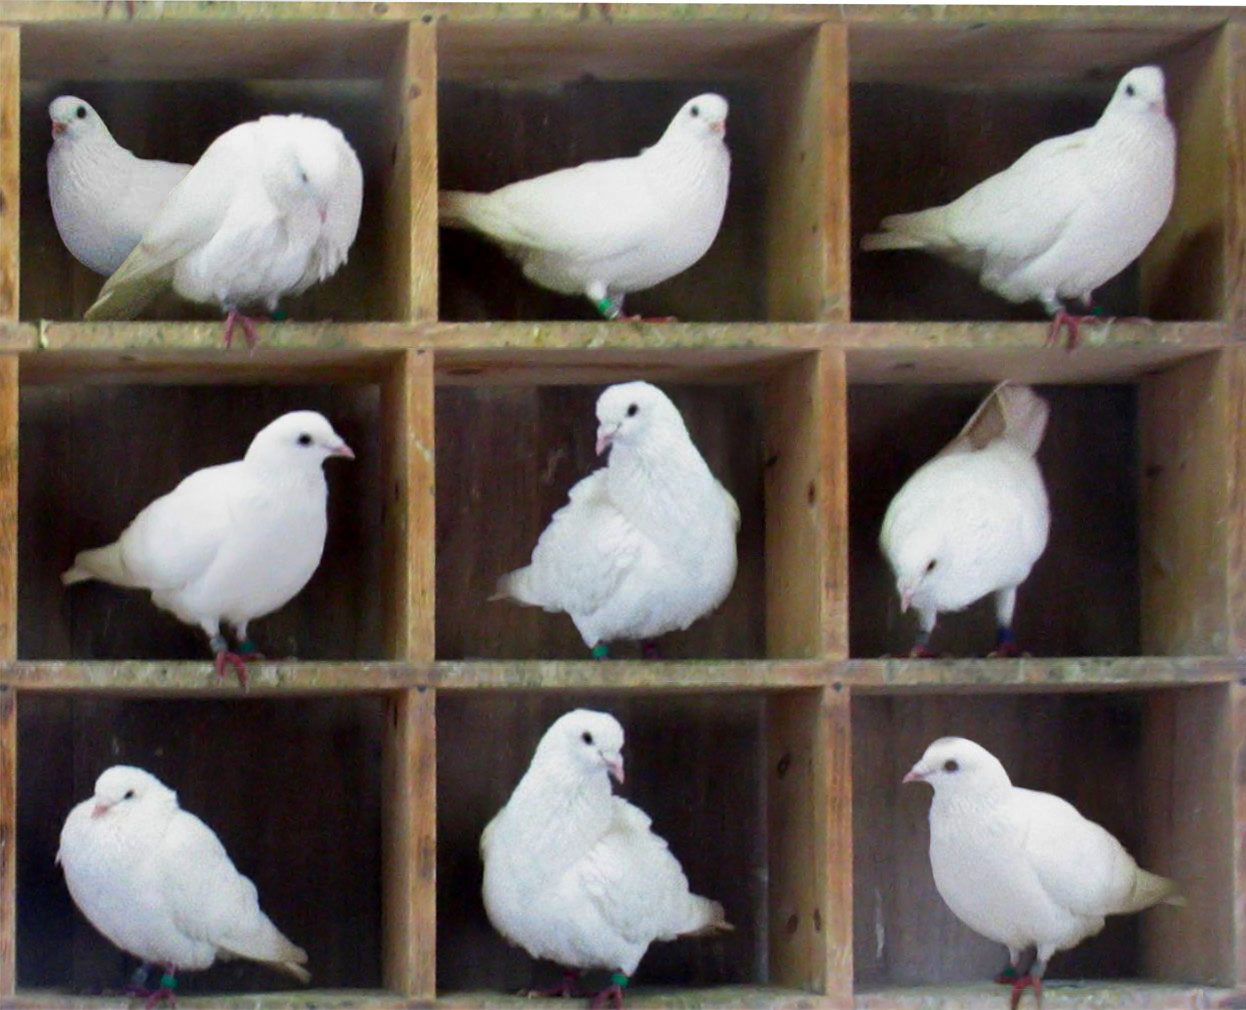
\includegraphics[height=180pt,width=\textwidth]{pictures/TooManyPigeons.jpg}%
	\caption*{We can think of separating complex entities as pigeonholing.}%
	\label{pigeonholing}%
\end{figure}%

Some aspects to take into account are:
\begin{enumerate}
    \item Can we refine the decision we need to a set of repetitive tasks where input information and output decision/value is well defined?
    \item Can we represent each sub-task we’ve defined with a mathematical mapping?
\end{enumerate}

The representation necessary for the second aspect may involve massaging of the problem: feature selection or adaptation. It may also involve filtering out exception cases (perhaps through a pre-classification).

All else being equal, we’d like to keep our models simple and interpretable. If we can convert a complex mapping to a linear mapping through clever selection of sub-tasks and features this is a big win.

For example, Facebook have \textit{feature engineers}, individuals whose main role is to design features they think might be useful for one of their tasks (e.g. newsfeed ranking, or ad matching). Facebook have a training/testing pipeline called FBLearner. Facebook have predefined the sub-tasks they are interested in, and they are tightly connected to their business model.

It is easier for Facebook to do this because their business model is heavily focused on user interaction. A challenge for companies that have a more diversified portfolio of activities driving their business is the identification of the most appropriate sub-task. A potential solution to feature and model selection is known as AutoML~\sidecite{Feurer2015EfficientAR}. Or we can think of it as using Machine Learning to assist Machine Learning. It’s also called meta-learning. Learning about learning. The input to the ML algorithm is a machine learning task, the output is a proposed model to solve the task.

One trap that is easy to fall in is too much emphasis on the type of model we have deployed rather than the appropriateness of the task decomposition we have chosen.

\textbf{Recommendation:} Conditioned on task decomposition, we should automate the process of model improvement. Model updates should not be discussed in management meetings, they should be deployed and updated as a matter of course. Further details below on model deployment, but model updating needs to be considered at design time. This is the domain of AutoML.

\begin{figure}[htbp]%
	
\includegraphics[height=180pt,width=\textwidth]{pictures/chicken-and-egg.jpg}%
	\caption*{The answer to the question which comes first, the chicken or the egg is simple, they co-evolve (\cite{Platnick1963ConjecturesAR}). Similarly, when we place components together in a complex machine learning system, they will tend to co-evolve and compensate for one another.}%
	\label{}%
\end{figure}%

To form modern decision making systems, many components are interlinked. We decompose our complex decision making into individual tasks, but the performance of each component is dependent on those upstream of it.

This naturally leads to co-evolution of systems, upstream errors can be compensated by downstream corrections.

To embrace this characteristic, end-to-end training could be considered. Why train individual systems by localized metrics when we can just optimize, globally, end-to-end for final system performance? End to end training can lead to improvements in performance, but it could also damage our systems decomposability, its interpretability, and perhaps its adaptability.

The less human interpretable our systems are, the harder they are to adapt to different circumstances or diagnose when there's a challenge. The trade-off between interpretability and performance is a constant tension which we should always retain in our minds when performing our system design.

\section{Data}

It is difficult to overstate the importance of data. It is half of the equation for machine learning, but is often utterly neglected. We can speculate that there are two reasons for this. Firstly, data cleaning is perceived as tedious. It doesn't seem to consist of the same intellectual challenges that are inherent in constructing complex mathematical models and implementing them in code. Secondly, data cleaning is highly complex, it requires a deep understanding of how machine learning systems operate and good intuitions about the data itself, the domain from which data is drawn (e.g. Supply Chain) and what downstream problems might be caused by poor data quality.

A consequence of these two reasons, data cleaning seems difficult to formulate into a readily teachable set of principles. As a result it is heavily neglected in courses on machine learning and data science. Despite data being half the equation, most University courses spend little to no time on its challenges.

However, these challenges aren't new, they are merely taking a different form.

Anecdotally, talking to data modelling scientists, most say they spend 80\% of their time acquiring and cleaning data. The “software crisis” was the inability to deliver software solutions due to increasing complexity of implementation. There was no single shot solution for the software crisis, it involved better practice (scrum, test orientated development, sprints, code review), improved programming paradigms (object orientated, functional) and better tools (CVS, then SVN, then git).

\section{The Software Crisis}
\begin{displayquote}
The major cause of the software crisis is that the machines have become several orders of magnitude more powerful! To put it quite bluntly: as long as there were no machines, programming was no problem at all; when we had a few weak computers, programming became a mild problem, and now we have gigantic computers, programming has become an equally gigantic problem.

Edsger Dijkstra (1930-2002), The Humble Programmer
\end{displayquote}

In the late sixties early software programmers made note of the increasing costs of software development and termed the challenges associated with it as the ``Software Crisis''. Edsger Dijkstra referred to the crisis in his 1972 Turing Award winner's address.

\section{The Data Crisis}

Modern software is driven by \textit{data}. That is the essence of machine learning. We can therefore see the software crisis as merely the first wave of a (perhaps) larger phenomenon, ``the data crisis''.

We can update Dijkstra's quote for the modern era.

\begin{displayquote}
The major cause of the data crisis is that machines have become more interconnected than ever before. Data access is therefore cheap, but data quality is often poor. What we need is cheap high quality data. That implies that we develop processes for improving and verifying data quality that are efficient.

There would seem to be two ways for improving efficiency. Firstly, we should not duplicate work. Secondly, where possible we should automate work.
\end{displayquote}

The quantity of modern data, and the lack of attention paid to data as it is initially "laid down" and the costs of data cleaning are bringing about a crisis in data-driven decision making. This crisis is at the core of the challenge of technical debt in machine learning \sidecite{Sculley2015HiddenTD}.

Just as with software, the crisis is most correctly addressed by 'scaling' the manner in which we process our data. Duplication of work occurs because the value of data cleaning is not correctly recognised in management decision making processes. Automation of work is increasingly possible through techniques in ``artificial intelligence'', but this will also require better management of the data science pipeline so that data about data science (meta-data science) can be correctly assimilated and processed. The Alan Turing institute has a program focused on this area, ``AI for Data Analytics''.

Data is the new software, and the data crisis is already upon us. It is driven by the cost of cleaning data, the paucity of tools for monitoring and maintaining our deployments, the provenance of our models (e.g. with respect to the data they’re trained on).

Three principal changes need to occur in response. They are cultural and infrastructural.

\subsection{The Data First Paradigm}

First of all, to excel in data driven decision making we need to move from a \textit{software first} paradigm to a \textit{data first} paradigm. That means refocusing on data as the product. Software is the intermediary to producing the data, and its quality standards must be maintained, but not at the expense of the data we are producing. Data cleaning and maintenance need to be prized as highly as software debugging and maintenance. Instead of \textit{software} as a service, we should refocus around \textit{data} as a service. This first change is a cultural change in which our teams think about their outputs in terms of data. Instead of decomposing our systems around the software components, we need to decompose them around the data generating and consuming components\footnote{Data Readiness Levels (\cite{Lawrence2017DataRL}) are an attempt to develop a language around data quality that can bridge the gap between technical solutions and decision makers such as managers and project planners. The are inspired by Technology Readiness Levels which attempt to quantify the readiness of technologies for deployment.}. Software first is only an intermediate step on the way to be coming \textit{data first}. It is a necessary, but not a sufficient condition for efficient machine learning systems design and deployment. We must move from \textit{software orientated architecture} to a \textit{data orientated architecture}.

\subsection{Data Quality}

Secondly, we need to improve our language around data quality. We cannot assess the costs of improving data quality unless we generate a language around what data quality means. Data Readiness Levels \sidecite{Lawrence2017DataRL} are an assessment of data quality that is based on the usage to which data is put.

\subsection{Move Beyond Software Engineering to Data Engineering}

Thirdly, we need to improve our mental model of the separation of data science from applied science. A common trap in current thinking around data is to see data science (and data engineering, data preparation) as a sub-set of the software engineer’s or applied scientist’s skill set. As a result we recruit and deploy the wrong type of resource. Data preparation and question formulation is superficially similar to both because of the need for programming skills, but the day to day problems faced are very different.

\textbf{Recommendation:} Build a shared understanding of the language of data readiness levels for use in planning documents, the costing of data cleaning, and the benefits of reusing cleaned data.

\section{Combining Data and Systems Design}

One analogy I find helpful for understanding the depth of change we need is the following. Imagine as a software engineer, you find a USB stick on the ground. And for some reason you \textit{know} that on that USB stick is a particular API call that will enable you to make a significant positive difference on a business problem. However, you also know on that USB stick there is potentially malicious code. The most secure thing to do would be to not introduce this code into your production system. But what if your manager told you to do so, how would you go about incorporating this code base?

The answer is \textit{very} carefully. You would have to engage in a process more akin to debugging than regular software engineering. As you understood the code base, for your work to be reproducible, you should be documenting it, not just what you discovered, but how you discovered it. In the end, you typically find a single API call that is the one that most benefits your system. But more thought has been placed into this line of code than any line of code you have written before.

Even then, when your API code is introduced into your production system, it needs to be deployed in an environment that monitors it. We cannot rely on an individual’s decision making to ensure the quality of all our systems. We need to create an environment that includes quality controls, checks and bounds, tests, all designed to ensure that assumptions made about this foreign code base are remaining valid.

This situation is akin to what we are doing when we incorporate data in our production systems. When we are consuming data from others, we cannot assume that it has been produced in alignment with our goals for our own systems. Worst case, it may have been adversarialy produced. A further challenge is that data is dynamic. So, in effect, the code on the USB stick is evolving over time.

Anecdotally, resolving a machine learning challenge requires 80\% of the resource to be focused on the data and perhaps 20\% to be focused on the model. But many companies are too keen to employ machine learning engineers who focus on the models, not the data.

\begin{figure}[htbp]%
	
\includegraphics[height=180pt,width=\textwidth]{pictures/water-bridge-hill-transport-arch.jpg}%
	\caption*{A reservoir of data has more value if the data is consumable. The data crisis can only be addressed if we focus on outputs rather than inputs.}%
	\label{water-bridge}%
\end{figure}%

\begin{figure}[htbp]%
	
\includegraphics[height=180pt,width=\textwidth]{pictures/Lake_District.JPG}%
	\caption*{For a data first architecture we need to clean our data at source, rather than individually cleaning data for each task. This involves a shift of focus from our inputs to our outputs. We should provide data streams that are consumable by many teams without purification.}%
	\label{lake-district}%
\end{figure}%

\textbf{Recommendation:} We need to share best practice around data deployment across our teams. We should make best use of our processes where applicable, but we need to develop them to become data first organizations. Data needs to be cleaned at output not at input.

\section{Deployment}

\subsection{Continuous Deployment}

Once the decomposition is understood, the data is sourced and the models are created, the model code needs to be deployed.

To extend our USB stick analogy further, how would we deploy that code if we thought it was likely to evolve in production? This is what datadoes. We cannot assume that the conditions under which we trained our model will be retained as we move forward, indeed the only constant we have is change.

This means that when any data dependent model is deployed into production, it requires \textit{continuous monitoring} to ensure the assumptions of design have not been invalidated. Software changes are qualified through testing, in particular a regression test ensures that existing functionality is not broken by change. Since data is continually evolving, machine learning systems require 'continual regression testing': oversight by systems that ensure their existing functionality has not been broken as the world evolves around them. An approach we refer to as \textit{progression testing}. Unfortunately, standards around ML model deployment yet been developed. The modern world of continuous deployment does rely on testing, but it does not recognize the continuous evolution of the world around us.

\textbf{Recommendation:} We establish best practice around model deployment. We need to shift our culture from standing up a software service, to standing up a \textit{data as a service}. Data as a Service would involve continual monitoring of our deployed models in production. This would be regulated by 'hypervisor' systems\footnote{Emulation, or surrogate modelling, is one very promising approach to forming such a hypervisor. Emulators are models we fit to other models, often simulations, but the could also be other machine learning models. These models operate at the meta-level, not on the systems directly. This means they can be used to model how the sub-systems interact. As well as emulators we should consider real time dash boards, anomaly detection, mutlivariate analysis, data visualization and classical statistical approaches for hypervision of our deployed systems.} that understand the context in which models are deployed and recognize when circumstance has changed and models need retraining or restructuring.

\textbf{Recommendation:} We should consider a major re-architecting of systems around our services. In particular we should scope the use of a \textit{streaming architecture} (such as Apache Kafka) that ensures data persistence and enables asynchronous operation of our systems\footnote{These approaches are one area of focus for my own team's research. A data first architecture is a prerequisite for efficient deployment of machine learning systems.}. This would enable the provision of QC streams, and real time dash boards as well as hypervisors.

Importantly a streaming architecture implies the services we build are \textit{stateless}, internal state is deployed on streams alongside external state. This allows for rapid assessment of other services' data.

\section{Outlook for Machine Learning}

Machine learning has risen to prominence as an approach to scaling our activities. For us to continue to automate in the manner we have over the last two decades, we need to make more use of computer-based automation. Machine learning is allowing us to automate processes that were out of reach before.

\section{Conclusion}

We operate in a technologically evolving environment. Machine learning is becoming a key component in our decision making capabilities. But the evolving nature of data driven systems means that new approaches to model deployment are necessary. We have characterized three parts of the machine learning systems design process. \textit{Decomposition} of the problem into separate tasks that are addressable with a machine learning solution. Collection and curation of appropriate \textit{data}. Verification of data quality through data readiness levels. Using \textit{progression} testing in our \textit{deployments}. Continuously updating models as appropriate to ensure performance and quality is maintained.

\chapter{Deploying Machine Learning:\\Intellectual Debt and AutoAI}

From the dawn of cybernetics, and across the last eight decades, we have worked to make machine learning methods successful. But now that these methods are being widely adopted we need to deal with the consequences of success. Many of those consequences can only be understood when a holistic approach to the machine learning problem is considered: the deployment of a method within a context for a particular objective. In this circumstance, it’s easy to see that questions of interpretability, fairness and transparency are all contextual. In this chapter we summarize this challenge using Jonathan Zittrain’s term of 'intellectual debt', we discuss how it pans out in reality and how this challenge could be addressed using machine learning techniques to give us 'Auto AI'.

\section{The Great AI Fallacy}

There is a lot of variation in the use of the term artificial intelligence. I’m sometimes asked to define it, but depending on whether you’re speaking to a member of the public, a fellow machine learning researcher, or someone from the business community, the sense of the term differs.

However, underlying its use I have detected one disturbing trend. A trend I’m beginning to think of as "The Great AI Fallacy".

The fallacy is associated with an implicit promise that is embedded in many statements about Artificial Intelligence. Artificial Intelligence, as it currently exists, is merely a form of automated decision making. The implicit promise of Artificial Intelligence is that it will be the first wave of automation where the machine adapts to the human, rather than the human adapting to the machine.

How else can we explain the suspension of sensible business judgment that is accompanying the hype surrounding AI?

This fallacy is particularly pernicious because there are serious benefits to society in deploying this new wave of data-driven automated decision making. But the AI Fallacy is causing us to suspend our calibrated skepticism that is needed to deploy these systems safely and efficiently.

The problem is compounded because many of the techniques that we’re speaking of were originally developed in academic laboratories in isolation from real-world deployment.

\begin{marginfigure}%
    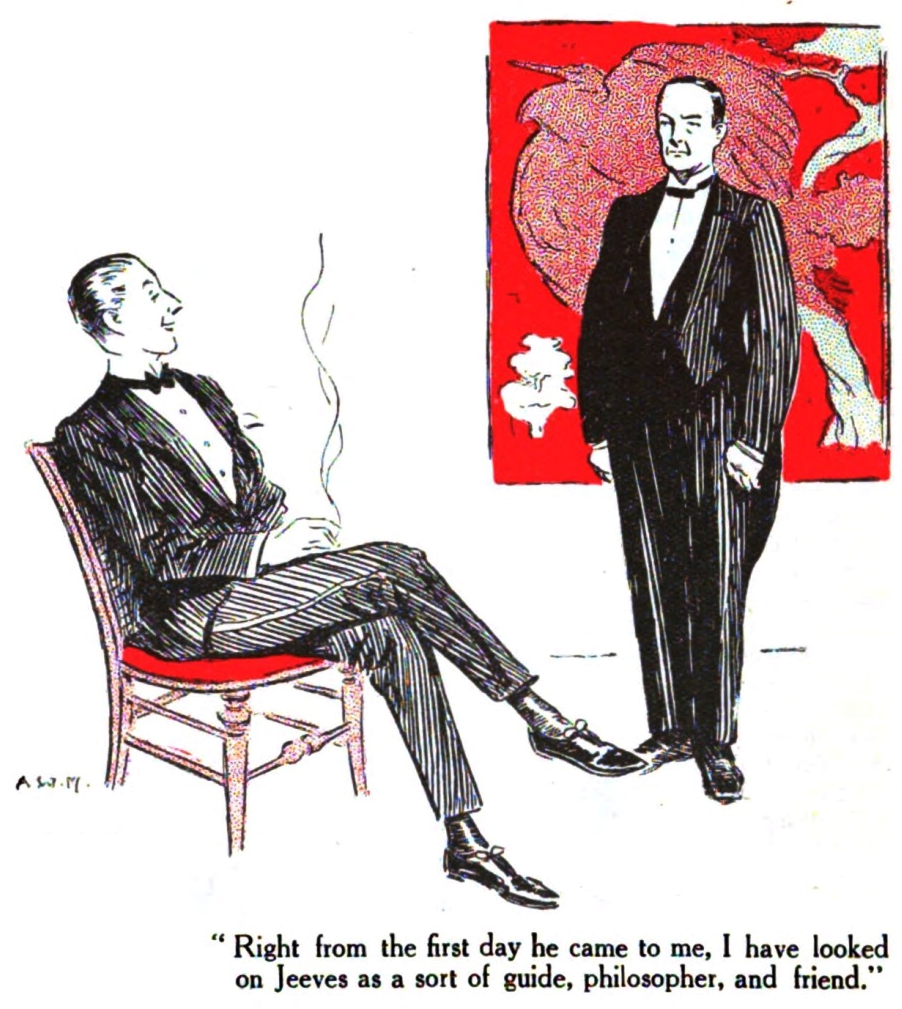
\includegraphics[width=\marginparwidth]{pictures/Jeeves_in_the_Springtime_01.jpg}%
    \caption*{We seem to have fallen for a perspective on AI that suggests it will adapt to our schedule, rather in the manner of a 1930s manservant.\label{rectangle}}%
\end{marginfigure}%

\section{Artificial vs Natural Systems}

Let’s take a step back from artificial intelligence, and consider natural intelligence. Or even more generally, let’s consider the contrast between an artificial system and an natural system. The key difference between the two is that artificial systems are designed whereas natural systems are evolved.

Systems design is a major component of all Engineering disciplines. The details differ, but there is a single common theme: achieve your objective with the minimal use of resources to do the job. That provides efficiency. The engineering designer imagines a solution that requires the minimal set of components to achieve the result. A water pump has one route through the pump. That minimises the number of components needed. Redundancy is introduced only in safety critical systems, such as aircraft control systems. Students of biology, however, will be aware that in nature system-redundancy is everywhere. Redundancy leads to robustness. For an organism to survive in an evolving environment it must first be robust, then it can consider how to be efficient. Indeed, organisms that evolve to be too efficient at a particular task, like those that occupy a niche environment, are particularly vulnerable to extinction.

This notion is akin to the idea that only the best will survive, popularly encoded into an notion of evolution by Herbert Spencer’s quote.

\begin{displayquote}
Survival of the fittest

Herbet Spencer, 1864
\end{displayquote}

Darwin himself never said ``Survival of the Fittest'' when he talked about evolution by natural selection.

Evolution is better described as ``non-survival of the non-fit''. You don’t have to be the fittest to survive, you just need to avoid the pitfalls of life. This is the first priority.

So it is with natural vs artificial intelligences. Any natural intelligence that was not robust to changes in its external environment would not survive, and therefore not reproduce. In contrast the artificial intelligences we produce are designed to be efficient at one specific task: control, computation, playing chess. They are \textit{fragile}.

The first rule of a natural system is not be intelligent, it is ``don’t be stupid''.

A mistake we make in the design of our systems is to equate fitness with the objective function, and to assume it is known and static. In practice, a real environment would have an evolving fitness function which would be unknown at any given time.

The first criterion of a natural intelligence is \textit{don’t fail}, not because it has a will or intent of its own, but because if it had failed it wouldn’t have stood the test of time. It would no longer exist. In contrast, the mantra for artificial systems is to be more efficient. Our artificial systems are often given a single objective (in machine learning it is encoded in a mathematical function) and they aim to achieve that objective efficiently. These are different characteristics. Even if we wanted to incorporate don’t fail in some form, it is difficult to design for. To design for "don’t fail", you have to consider every which way in which things can go wrong, if you miss one you fail. These cases are sometimes called corner cases. But in a real, uncontrolled environment, almost everything is a corner. It is difficult to imagine everything that can happen. This is why most of our automated systems operate in controlled environments, for example in a factory, or on a set of rails. Deploying automated systems in an uncontrolled environment requires a different approach to systems design. One that accounts for uncertainty in the environment and is robust to unforeseen circumstances.

\section{Intellectual Debt}

\begin{figure}[htbp]%
	
\includegraphics[width=\textwidth,keepaspectratio]{pictures/2020-02-12-intellectual-debt.png}%
	\caption*{Jonathan Zittrain’s term to describe the challenges of explanation that come with AI is Intellectual Debt.}%
	\label{intellectual-debt}%
\end{figure}%

In computer systems the concept of \textit{technical debt} has been surfaced by authors including Sculley et al.\sidecite{Sculley2015HiddenTD}. It is an important concept, that I think is somewhat hidden from the academic community, because it is a phenomenon that occurs when a computer software system is deployed.

\subsection{Separation of Concerns}

To construct such complex systems an approach known as ``separation of concerns'' has been developed. The idea is that you architect your system, which consists of a large-scale complex task, into a set of simpler tasks. Each of these tasks is separately implemented. This is known as the decomposition of the task.

This is where Jonathan Zittrain’s beautifully named term ``intellectual debt'' rises to the fore. Separation of concerns enables the construction of a complex system. But who is concerned with the overall system?

\begin{itemize}
    \item Technical debt is the inability to \textit{maintain} your complex software system.
    \item Intellectual debt is the inability to \textit{explain} your software system.
\end{itemize}

It is right there in our approach to software engineering. ``Separation of concerns'' means no one is concerned about the overall system itself.

\subsection{Buying System}

An example of a complex decision making system might be an automated buying system. In such a system, the idea is to match demand for products to supply of products.

The matching of demand and supply is a repetetive theme for decision making systems. Not only does it occur in automated buying, but also in the allocation of drivers to riders in a ride sharing system. Or in the allocation of compute resource to users in a cloud system.

The components of any of these system include: predictions of the demand for the product, or the drivers or the compute. Then predictions of the supply. Decisions are then made for how much material to keep in stock, or how many drivers to have on the road, or how much computer capacity to have in your data centres. These decisions have cost implications. The optimal amount of product will depend on the cost of making it available. For a buying system this is the storage costs.

Decisions are made on the basis of the supply and demand to make new orders, to encourage more drivers to come into the system or to build new data centers or rent more computational power.

\begin{figure}[htbp]%
	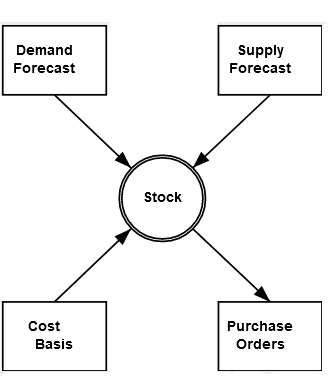
\includegraphics[width=0.6\textwidth,keepaspectratio]{pictures/buying_1.PNG}%
	\caption*{The components of a putative automated buying system.}%
% 	\label{rectangle2}%
\end{figure}%

\subsection{Monolithic System}

The classical approach to building these systems was a ‘monolithic system’. Built in a similar way to the successful applications software such as Excel or Word, or large operating systems, a single code base was constructed. The complexity of such code bases run to many lines.

In practice, shared dynamically linked libraries may be used for aspects such as user interface, or networking, but the software often has many millions of lines of code. For example, the Microsoft Office suite is said to contain over 30 millions of lines of code.

\begin{figure}[htbp]%
	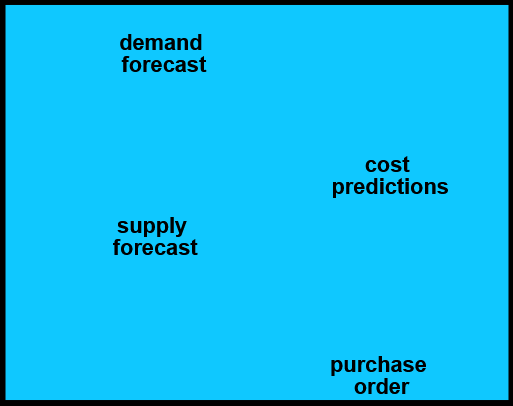
\includegraphics[width=0.6\textwidth,keepaspectratio]{pictures/buying_2.PNG}%
	\caption*{A potential path of models in a monolithic machine learning system.}%
% 	\label{rectangle2}%
\end{figure}%

\subsection{Service Oriented Architecture}

Such software is not only difficult to develop, it is difficult to scale when computation demands increase. Amazon’s original website software (called Obidos) was a monolithic design but by the early noughties it was becoming difficult to sustain and maintain. The software was phased out in 2006 to be replaced by a modularized software known as a ‘service oriented architecture’.

In Service Oriented Architecture the idea is that code bases are modularized and communicate with one another using network requests. A standard approach is to use a REST API. So, rather than a single monolithic code base, the code is developed with individual services that handle the different requests.

\begin{figure}[htbp]%
	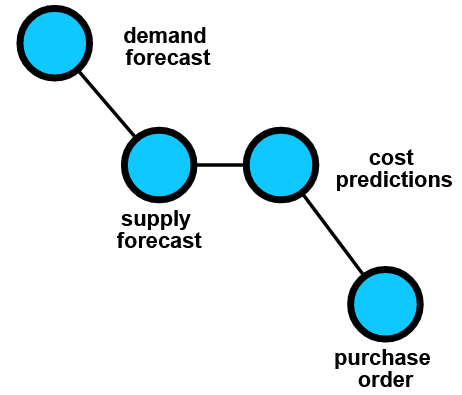
\includegraphics[width=0.6\textwidth,keepaspectratio]{pictures/buying_3.PNG}%
	\caption*{A potential path of models in a service-oriented machine learning system.}%
% 	\label{rectangle2}%
\end{figure}%

This is the landscape we now find ourselves in with regard to software development. In practice, each of these services is often ‘owned’ and maintained by an individual team. The team is judged by the quality of their service provision. They work to detailed specifications on what their service should output, what its availability should be and other objectives like speed of response. This allows for conditional independence between teams and for faster development.

\subsection{Buying to Banking}

The same model we consider for buying, can also be considered in the case of, for example, a banking application. In a typical banking application, we receive loan requests from customers. For an individual customer, before making a loan, the bank may wish to make a forecast around their costs (expenditures on food, housing, entertainment etc) and their income (salary, rental income etc). These forecasts would inform the conditions of the loan. For example how much the bank is willing to lend, and under what interest rates and repayment conditions. These terms will be based on previous experience of loaning, but also constrained by regulatory conditions often imposed by a financial regulator.

\begin{figure}[htbp]%
	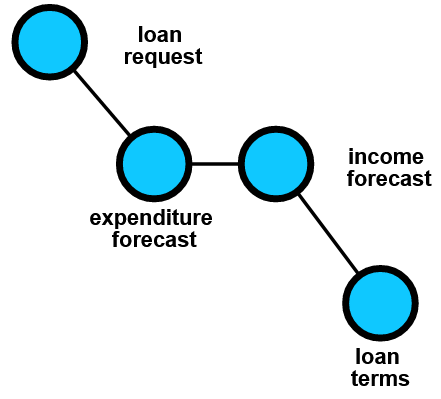
\includegraphics[width=0.6\textwidth,keepaspectratio]{pictures/banking_1.PNG}%
	\caption*{A potential path of models in a machine learning system where a decision about a loan is being made on the basis of (potentially personal) data from a customer.}%
% 	\label{rectangle2}%
\end{figure}%

In many regulatory environments, the bank will be restricted in terms of what information they are allowed to use in dictating loan terms. For example, with in the EU there are prohibited characteristics such as race, gender, sexuality, religion and health status which cannot be used (even indirectly) for making the loan. Along with stipulating these characteristics, the badly-named GDPR\footnote{The GDPR is "General Data Protection Regulation" but it does not ‘protect data’ it ‘protects individuals’ with regard to decision making based on their personal data. The misnomer data-protection is unfortunate, a better way of viewing this legislation is "personal data rights" legislation.} also gives particular stipulations for rights individuals have for explanation around consequential decisions, such as obtaining a loan.

The challenge of Intellectual Debt means that it’s possible for a bank to produce an automated loan decision system, which even the bank itself doesn’t understand, which makes it rather hard to conform to the intent of the GDPR which requires the bank to explain to customers the reasoning behind decisions based on personal data.

\subsection{SafeBoda}

The complexity of building safe, maintainable systems that are based on interacting components which include machine learning models means that smaller companies can be excluded from access to these technologies due the technical and intellectual debt incurred when maintaining such systems in a real-world environment.

\begin{figure}%
	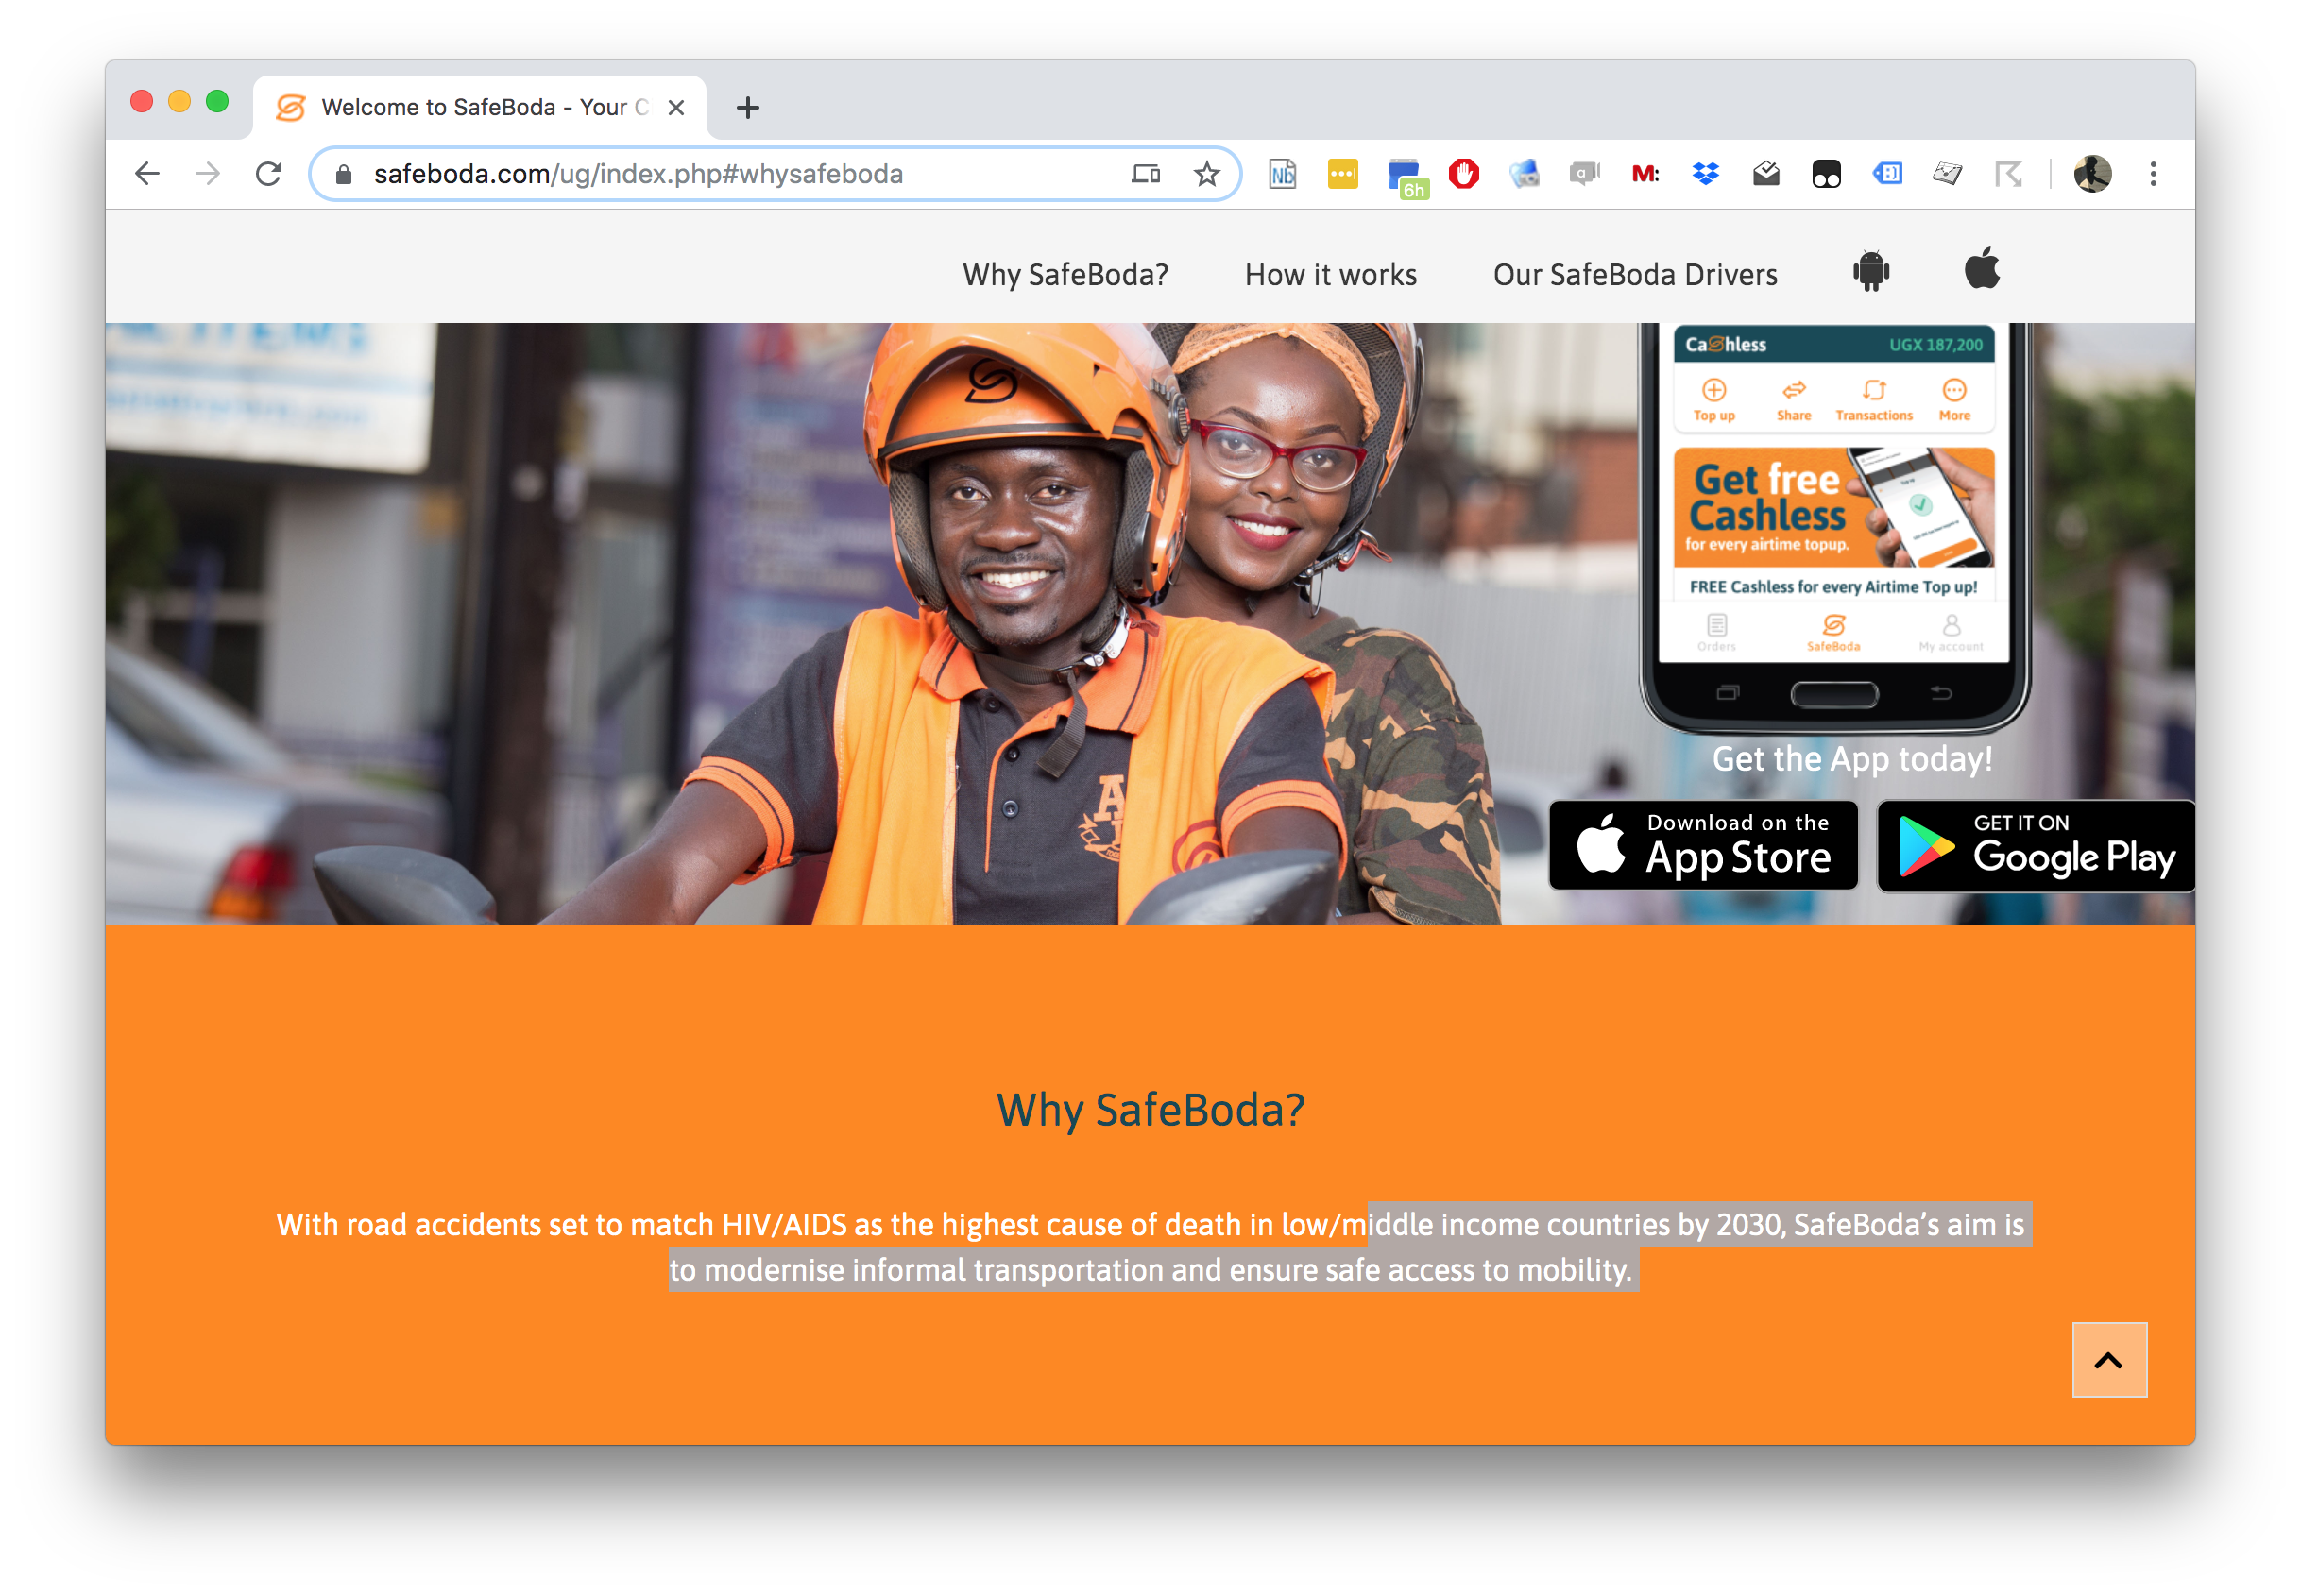
\includegraphics[width=0.6\textwidth,keepaspectratio]{pictures/safe-boda.png}%
	\caption*{SafeBoda is a ride allocation system for Boda Boda drivers. Let’s imagine the capabilities we need for such an AI system.}%
% 	\label{rectangle2}%
\end{figure}%

SafeBoda is a Kampala based rider allocation system for Boda Boda drivers. Boda boda are motorcycle taxis which give employment to, often young men, across Kampala. Safe Boda is driven by the knowledge that road accidents are set to match HIV/AIDS as the highest cause of death in low/middle income families by 2030.

\begin{displayquote}
With road accidents set to match HIV/AIDS as the highest cause of death in low/middle income countries by 2030, SafeBoda’s aim is to modernise informal transportation and ensure safe access to mobility.
\end{displayquote}

A key aim of the AutoAI agenda is to reduce these technical challenges, so that such software can be maintained safely and reliably by a small team of software engineers. Without this capability it is hard to imagine how low resource environments can fully benefit from the ‘data revolution’ without heavy reliance on technical provision from high-resource environments. Such dependence would inevitably mean a skew towards the challenges that high-resource economies face, rather than the more urgent and important problems that are faced in low-resource environments.

\subsection{FIT Models to FIT Systems}

Zittrain points out the challenge around the lack of interpretability of individual ML models as the origin of intellectual debt. In machine learning I refer to work in this area as fairness, interpretability and transparency or FIT models. To an extent I agree with Zittrain, but if we understand the context and purpose of the decision making, I believe this is readily put right by the correct monitoring and retraining regime around the model. A concept I refer to as ``progression testing''. Indeed, the best teams do this at the moment, and their failure to do it feels more of a matter of technical debt rather than intellectual, because arguably it is a maintenance task rather than an explanation task. After all, we have good statistical tools for interpreting individual models and decisions when we have the context. We can linearise around the operating point, we can perform counterfactual tests on the model. We can build empirical validation sets that explore fairness or accuracy of the model.

So, this is where, my understanding of intellectual debt in ML systems departs, I believe from John Zittrain’s. The long-term challenge is not in the individual model. We have excellent statistical tools for validating what any individual model, the long-term challenge is the complex interaction between different components in the decomposed system, where the original intent of each component has been forgotten (except perhaps by Lancelot) and each service has been repurposed. We need to move from FIT models to FIT systems.

How to address these challenges? With collaborators I have been working towards a solution that contains broadly two parts. The first part is what we refer to as ``Data-Oriented Architectures''. The second part is ``meta modelling'', machine learning techniques that help us model the models.

\begin{figure}%
	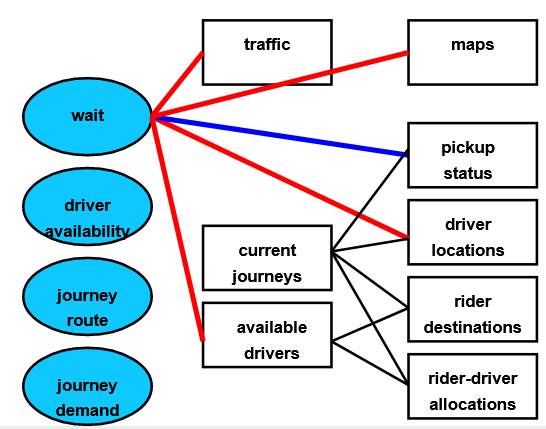
\includegraphics[width=0.6\textwidth,keepaspectratio]{pictures/boda_1.PNG}%
	\caption*{Some software components in a ride allocation system. Circled components are hypothetical, rectangles represent actual data.}%
% 	\label{rectangle2}%
\end{figure}%

\section{A Solution}

\subsection{Data-oriented Architectures}

Data-oriented architectures aim to address the rat’s nest that is the current interaction between the services in a service-oriented architecture. It does this by introducing data-oriented programming. The data-oriented programming language tracks the movement of data between each service.

Service-oriented programming style is a necessary, but not sufficient approach to data-oriented programming. Data-oriented programming is not only about the individual services, but how they are connected. Which service is calling which and where the flow of the data through the system occurs?

If each service has its inputs and outputs declared on a wider ecosystem, then we can programmatically determine which inputs effect which decisions. This programmatic discovery is vital because as systems are built compositionally, the actual inputs that affect a final decision may not be known to any of the software engineers who are maintaining the system.

\subsection{Milan}

To answer these challenges at Amazon we began the process of constructing software for data oriented architectures. The team built a \textit{data-oriented programming} language which is now available\footnote{https://github.com/amzn/milan} through Apache 2.0 license. The language is called Milan. Quoting from Tom Borchert’s blog on Milan:

\begin{displayquote}
Milan has three components:

\begin{enumerate}
    \item A general-purpose stream algebra that encodes relationships between data streams (the Milan Intermediate Language or Milan IL).
    \item A Scala library for building programs in that algebra.
    \item A compiler that takes programs expressed in Milan IL and produces a Flink application that executes the program.
\end{enumerate}
        
Component (2) can be extended to support interfaces in additional languages, and component (3) can be extended to support additional runtime targets. Considering just the multiple interfaces and the multiple runtimes, Milan looks a lot like the much more mature Apache Beam. The difference lies in (1), Milan’s general-purpose stream algebra.
\end{displayquote}

It is through the general-purpose stream algebra that we hope to make significant inroads on the intellectual debt challenge.

The stream algebra defines the relationship between different machine learning components in the wider software architecture. Composition of multiple services cannot occur without a signature existing within the stream algebra. The Milan IL becomes the key information structure that is required to reason about the wider software system.

\subsection{Context}

This deals with the challenges that arise through the intellectual debt because we can now see the context around each service. This allows us to design the relevant validation checks to ensure that accuracy and fairness are maintained. By recompiling the algebra to focus on a particular decision within the system we can also derive new statistical tests to validate performance. These are the checks that we refer to as progression testing. The loss of programmer control means that we can no longer rely on software tests written at design time, we must have the capability to deploy new (statistical) tests after deployment as the uses to which each service is placed extend to previously un-envisaged domains.

\subsection{Stateless Services}

Importantly, Milan does not place onerous constraints on the builders of individual machine learning models (or other components). Standard modelling frameworks can be used. The main constraint is that any code that is not visible to the ecosystem does not maintain or store global state. This condition implies that the parameters of any machine learning model need to also be declared as an input to the model within the Milan IL.

\subsection{Meta Modelling}

Where does machine learning come in? The strategy I propose is that the Milan IL is integrated with meta-modelling approaches to assist in the explanation of the decision-making framework. At their simplest these approaches may be novelty detection algorithms on the data streams that are emerging from a given service. This is a form of progression testing. But we can go much further. By knowing the training data, the inputs and outputs of the individual services in the software ecosystem, we can build meta-models that test for fairness, accuracy not just of individual system components, but short or long cascades of decision making. Through the use of the Milan IL algebra all these tests could be automatically deployed. The focus of machine learning is on the models-that-model-the-models. The meta-models.

In Amazon, our own focus was on the use of statistical emulators, sometimes known as surrogate models, for fulfilling this task. The work we were putting into this route is available through another software package, Emukit\sidecite{emukit2019}, a framework for decision making under uncertainty. With collaborators my current focus for addressing these issues is a form of fusion of Emukit and Milan (Milemukit??). But the nature of this fusion requires testing on real world problem sets. A task we hope to carry out in close collaboration with colleagues at Data Science Africa.

\subsection{AutoAI: FIT Models to FIT Systems}

The idea of AutoAI is to combine the streaming algebra we obtain from the data oriented architecture (we can think of it as a ‘tube map for data flows’) with monitoring techniques both from machine learning, classical statistics and softare verification for ensuring that the system is performing as designed and/or alerting us to when our assumptions about the system are invalidated.

We can already deploy classical statistical approaches for e.g. outlier detection, or use proofs from category theory to demonstrate that a particular decision is not based on a protected characteristic.

The additional aim would be to use techniques from uncertainty quantification and statistical emulation to provide more interpretability to those decisions.

This domain has been called FAT modelling in machine learning, but I prefer the acronym FIT for fairness, interpretability and transparency.

AutoAI makes us realise that AutoML isn’t sufficient for improving the performance of the system, because it works on a componentwise basis. Similarly, FIT machine learning models are not sufficient. We need to move from FIT models to FIT systems.

\subsection{Statistical Emulation}

\begin{figure}%
	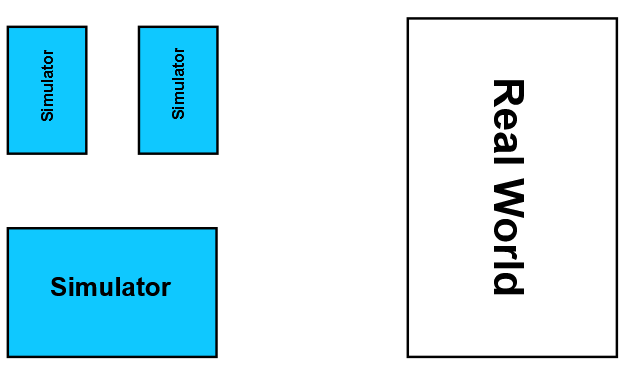
\includegraphics[width=0.6\textwidth,keepaspectratio]{pictures/sim_1.PNG}%
	\caption*{Real world systems consiste of simulators, that capture our domain knowledge about how our systems operate. Different simulators run at different speeds and granularities.}%
% 	\label{rectangle2}%
\end{figure}%

In many real world systems, decisions are made through simulating the environment. Simulations may operate at different granularities. For example, simulations are used in weather forecasts and climate forecasts. The UK Met office uses the same code for both, but operates climate simulations one at greater spatial and temporal resolutions.

\begin{figure}%
	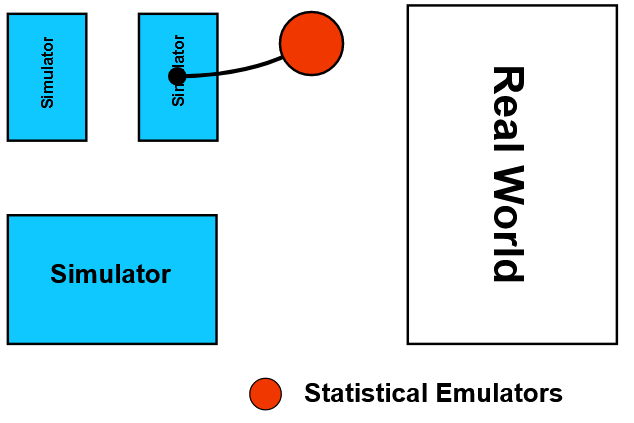
\includegraphics[width=0.6\textwidth,keepaspectratio]{pictures/sim_2.PNG}%
	\caption*{A statistical emulator is a system that reconstructs the simulation with a statistical model.}%
% 	\label{rectangle2}%
\end{figure}%

A statistical emulator is a data-driven model that learns about the underlying simulation. Importantly, learns with uncertainty, so it ‘knows what it doesn't know’. In practice, we can call the emulator in place of the simulator. If the emulator ‘doesn't know’, it can call the simulator for the answer.

\begin{figure}%
	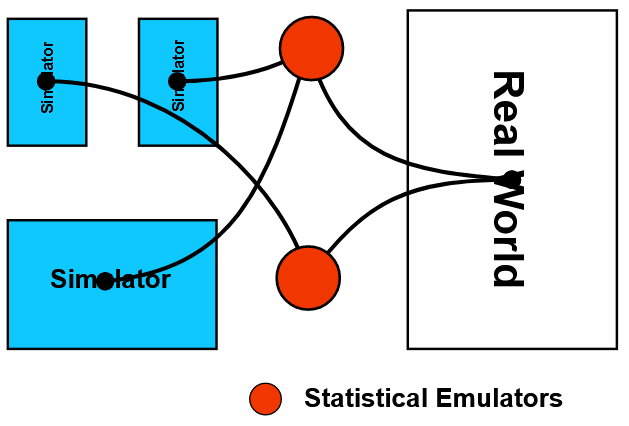
\includegraphics[width=0.6\textwidth,keepaspectratio]{pictures/sim_3.PNG}%
	\caption*{A statistical emulator is a system that reconstructs the simulation with a statistical model. As well as reconstructing the simulation, a statistical emulator can be used to correlate with the real world.}%
% 	\label{rectangle2}%
\end{figure}%

\begin{figure}%
	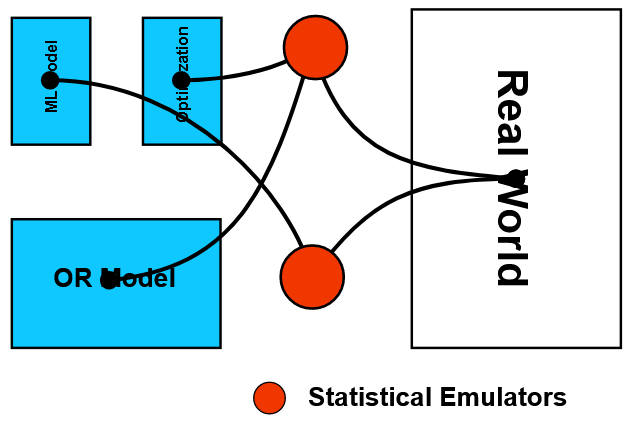
\includegraphics[width=0.6\textwidth,keepaspectratio]{pictures/sim_4.PNG}%
	\caption*{In modern machine learning system design, the emulator may also consider the output of ML models (for monitoring bias or accuracy) and Operations Research models.}%
% 	\label{rectangle2}%
\end{figure}%

As well as reconstructing an individual simulator, the emulator can calibrate the simulation to the real world, by monitoring differences between the simulator and real data. This allows the emulator to characterise where the simulation can be relied on, i.e. we can validate the simulator.

Similarly, the emulator can adjudicate between simulations. This is known as multi-fidelity emulation. The emulator characterizes which emulations perform well where.

If all this modelling is done with judicious handling of the uncertainty, the computational doubt, then the emulator can assist in deciding what experiment should be run next to aid a decision: should we run a simulator, in which case which one, or should we attempt to acquire data from a real world intervention.

\subsection{Deep Emulation}

As a solution we can use of emulators. When constructing an ML system, software engineers, ML engineers, economists and operations researchers are explicitly defining relationships between variables of interest in the system. That implicitly defines a joint distribution, $p(y^{*},y)$. In a decomposable system any sub-component may be defined as $p(y_i|y_j)$ where $y_i$ and $y_j$ represent sub-sets of the full set of variables ${y^{*},y}$. In those cases where the relationship is deterministic, the probability density would collapse to a vector-valued deterministic function, $f_i(y_j)$.

Inter-variable relationships could be defined by, for example a neural network (machine learning), an integer program (operational research), or a simulation (supply chain). This makes probabilistic inference in this joint density for real world systems is either very hard or impossible.

Emulation is a form of meta-modelling: we construct a model of the model. We can define the joint density of an emulator as $s(y^{*},y)$, but if this probability density is to be an accurate representation of our system, it is likely to be prohibitively complex. Current practice is to design an emulator to deal with a specific question. This is done by fitting an ML model to a simulation from the appropriate conditional distribution, $p(y_i|y_j)$, which is intractable. The emulator provides an approximated answer of the form $s(y_i|y_j)$. Critically, an emulator should incorporate its uncertainty about its approximation. So the emulator answer will be less certain than direct access to the conditional $p(y_i|y_j)$, but it may be sufficiently confident to act upon. Careful design of emulators to answer a given question leads to efficient diagnostics and understanding of the system. But in a complex interacting system an exponentially increasing number of questions can be asked. This calls for a system of automated construction of emulators which selects the right structure and redeploys the emulator as necessary. Rapid redeployment of emulators could exploit pre-existing emulators through \textit{transfer learning}.

Automatically deploying these families of emulators for full system understanding is highly ambitious. It requires advances in engineering infrastructure, emulation and Bayesian optimization. However, the intermediate steps of developing this architecture also allow for automated monitoring of system accuracy and fairness. This facilitates AutoML on a component-wise basis which we can see as a simple implementation of AutoAI. The proposal is structured so that despite its technical ambition there is a smooth ramp of benefits to be derived across the programme of work.

In Applied Mathematics, the field studying these techniques is known as \textit{uncertainty quantification}. The new challenge is the automation of emulator creation on demand to answer questions of interest and facilitate the system design, i.e. AutoAI through BSO.

At design stage, any particular AI task could be decomposed in multiple ways. Bayesian system optimization will assist both in determining the large-scale system design through exploring different decompositions and in refinement of the deployed system.

So far, most work on emulators has focused on emulating a single component. Automated deployment and maintenance of ML systems requires networks of emulators that can be deployed and redeployed on demand depending on the particular question of interest. Therefore, the technical innovations we require are in the mathematical composition of emulator models \sidecite{damianou2013deep, Perdikaris2017NonlinearIF}. Different chains of emulators will need to be rapidly composed to make predictions of downstream performance. This requires rapid retraining of emulators and \textit{propagation of uncertainty} through the emulation pipeline a process we call \textit{deep emulation}.

Recomposing the ML system requires structural learning of the network. By parameterizing covariance functions appropriately this can be done through Gaussian processes \sidecite{damianou2012manifold}, but one could also consider Bayesian neural networks and other generative models, e.g. Generative Adversarial Networks \sidecite{Goodfellow2014GenerativeAN}.

\begin{figure}%
	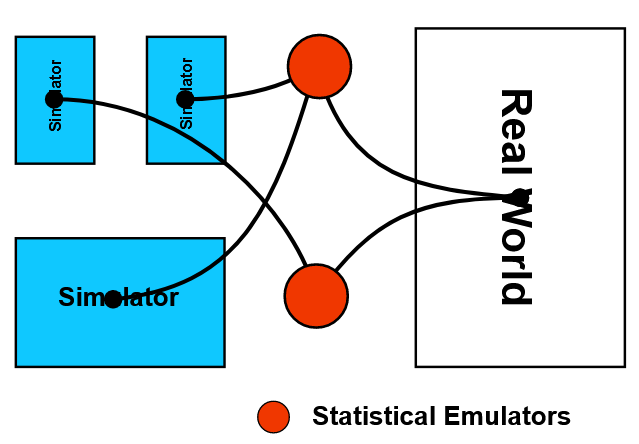
\includegraphics[width=0.6\textwidth,keepaspectratio]{pictures/sim_5.PNG}%
	\caption*{A statistical emulator is a system that reconstructs the simulation with a statistical model. As well as reconstructing the simulation, a statistical emulator can be used to correlate with the real world.}%
% 	\label{rectangle2}%
\end{figure}%

\section{Conclusion}

Today’s artificial intelligence is fundamentally Machine Learning Systems design, but the systems we are building will not fulfill the promises we are making for them (The Great AI Fallacy). We are not yet ready to deploy automation in fully uncontrolled environments due to major issues around intellectual debt. Until we modify our approaches we will not be able to deliver on the promise. Until then, monitoring and update of deployed systems will be key to practical and safe AI.

\chapter{Storming the Castle:\\Data science for COVID-19 Policy}

In the classic film Monty Python and the Holy Grail, John Cleese, as Sir Lancelot the Brave, finds a note – a plea from a prisoner of Swamp Castle – beseeching the discoverer to help them escape an unwanted marriage. Responding to this distress call, Sir Lancelot singlehandedly storms Swamp Castle, slaying the guards, terrorising the wedding guests, and fighting his way to the Tall Tower. There, instead of the expected damsel in distress, cruelly imprisoned, Sir Lancelot is surprised to find a wayward groom, Prince Herbert, who sent the note after an argument with his father.

The United Kingdom is considered an international leader in science, and a pioneer in the provision of science advice. The Government has well-established structures for accessing scientific expertise in emergencies through its network of science advisers, the Scientific Advisory Group for Emergencies (SAGE) and departmental advisory committees, including the Science for Pandemic Influenza Groups that provide advice on COVID-19 modelling and behavioural science. Together, these structures might call to mind a different Arthurian vision, evoking the works of Thomas Malory: the scientist as Merlin, giving wise counsel to Arthur and honing the Government’s decision-making through deep knowledge of the scientific arts.

Scientists are concerned citizens, and it is perhaps with this vision of adviser as trusted arbiter that many researchers entered into public and policy debates surrounding COVID-19. While pursuing the wise Merlin, however, efforts to advise government can easily drift towards Monty Python’s Lancelot. Confident in his knowledge of castle-storming, his individual dedication and his skills in damsel-rescuing, Sir Lancelot enters the fray with only a partial understanding of the challenges and circumstances at hand.

Science policy has long sought ways of bridging the gaps between scientists and policymakers, helping each understand the ways in which evidence can inform policymaking. The UK’s response to the COVID-19 pandemic has highlighted the importance of this work, and the long-standing cultural issues that make this mission so challenging. Driven by experiment and theory, scientists often seek definitive answers to a particular question, with each new study prompting more questions and illuminating areas for investigation that stretch into the future. In contrast, policy advice is often rooted to a moment in time. Events cannot wait for definitive scientific understanding. Instead, policymakers need access to high-quality advice that provides actionable insights, based on current understandings, while acknowledging areas of uncertainty.

But what constitutes the best current understanding? Any policy issue can be viewed through multiple lenses: the scientific principles at hand, the economic implications, public acceptability of potential responses, the values embedded in those responses, or operational considerations in policy delivery, amongst others. Each of these lenses is important in considering the evidence available to inform responses to the COVID-19 pandemic: the complexity of the pandemic, our relatively limited understanding of the virus, and the practical difficulties of implementing public health policy demand a range of expertise.

These complex and uncertain challenges require a multi-disciplinary response.

The unprecedented nature of the pandemic has spurred multiple efforts to bring research expertise to bear on COVID-19 policymaking. These have included a call for rapid assistance from the modelling community, a group providing rapid review and literature analysis, and an independently convened SAGE group. Our own experience is of another of these efforts – the Royal Society-convened DELVE Initiative.

In the early stage of the pandemic, as many governments struggled to implement policies that held back the first wave of infections, data scientists began to explore how advanced analytics could complement traditional forms of government science advice. Chaired by the President of the Royal Society and feeding into SAGE, the DELVE Initiative set out to analyse data from countries at a more advanced stage of the COVID-19 pandemic, using these insights to inform UK policy responses.

Data science for ‘real world’ policy questions can only be done effectively with access to domain expertise: extracting insights from data is important, but applying these insights to policy development requires the contextual understanding brought by domain experts, including those embedded in the policymaking process. Mapping this onto the attack of Swamp Castle, Professor Lancelot is better advised to consult his colleagues at the Round Table before charging the Tall Tower – while Lancelot has the tools to break down the doors, other knights may know the residents, the routes in, and why the distress call was sent.

Bridging the ‘supply chain of ideas’ between researchers and policymakers has been core to DELVE’s approach. The breadth of COVID-19’s impacts and potential policy responses has required that DELVE make connections across public health, economics, behavioural science, immunology, and more, and the value of collaboration can be seen across DELVE reports. For example, in an early report on testing and tracing systems\sidecite{delve2020test}: researchers from public health brought a wealth of insights about how to detect and manage disease outbreaks in communities, data scientists translated this to analysis that quantified the compliance rates needed to ensure testing and tracing efforts would be successful, and economists contextualised this with evidence about what interventions would encourage individuals and organisations to comply with a test, trace, isolate regime. DELVE’s remit became interdisciplinary by default, with data the focal point around which to convene domain experts.

This type of evidence synthesis would traditionally rely on collaborations developed with the luxury of time – time to understand how different disciplines frame an issue and to identify the different types of evidence that might be policy-relevant. Using data as a convenor has offered a short-cut through these discussions, by creating a common focal point from which different domain experts can explore their ideas. Arthur brought his knights together through the convening power of a sword, Excalibur; DELVE convened its scientists through data.

Despite its importance in enabling rapid evidence synthesis, in pursuing this ambitious research agenda, a consistent barrier to further action has been access to data. Labouring the parallels to Arthurian legend, in many cases relevant data was so difficult to identify and access it may as well have been mythical. But in practice it was the idea that the data might exist and be accessible, rather its actual availability, that was sufficient to convene expertise through DELVE.

Barriers to government data sharing – whether resulting from perceived legal issues, lack of capability in government, or technical barriers to data use – were well-characterised before the pandemic, but have been thrown into sharp relief in recent months. Where successful data sharing arrangements have been established to support the COVID-19 response, these have tended to rely on pre-existing relationships between data scientists and policymakers that foster shared understandings of how to use data in research and policy. In some ways, other disciplines have already learned this lesson – sustained engagement between government and academia has played a central role in major policy changes across government, from the smoking ban to the Climate Change Act. If data science is to find a role in policymaking, it will need to build on these experiences.

A new model of open data science, which capitalises on the power of data in convening multidisciplinary exchanges, will be vital, if we are to realise the potential of data science for research and policy. By building a community of researchers at the interface of data science and other disciplines, there is an opportunity to create exciting new research agendas that both advance data science methods and generate new insights for research and policy. Such a community would embed multidisciplinary engagement in its research culture, developing relationships and building capacity for rapid response to future policy challenges. It would seek to create a governance environment in which data can be used safely and rapidly, while ensuring that data analysis tools are made widely available, with clear information about how to use them.

This open data science model will be central to the work of the Accelerate Programme for Scientific Discovery, a new initiative from the Cambridge Computer Lab that will pursue research at the interface of machine learning and the sciences. By operating outside the traditional boundaries that separate disciplines, open data science could bridge the gap between ‘data science’ and the domains that would benefit from its tools and techniques, enabling ideas to spread rapidly and ultimately advancing scientific discovery for the benefit of society.



% % The first chapter with annotation and citations
% \chapter{Quick start}
% %
% We compiled a minimal example file to show the basic use of the caesar class, which allows the typesetting of (science) textbooks or theses. The class itself is a reference implementation of the \emph{sidenotes} package. The package provides the additional functionality\sidenote{namely the use of marginal material such as this note or even figures or tables.} and the class gives sensible default values for page margins, chapter formatting and such. The caesar class is derived from the standard \LaTeX-book class and a little bit of experience with the standard class might be very helpful. In this example, biblatex is used for the references.

% The first pages of the book (the frontmatter) are not numbered, the numbering starts after the \texttt{mainmatter} macro, which is called after the generation of the title page. The layout has ample margins to allow annotations. A main feature and the package is the sidenote, which is a footnote in the margin and can be placed with the \texttt{sidenote} macro.\sidenote{All information is on the same page, no turning of pages is necessary.} It is very similar to \texttt{footnote} and tries to emulate its behavior. The sidenote moves up or down (floats) to not overlap with other floats in the margin and all the sidenotes are subsequently numbered. 

% References can be put in the margin as well.\sidecite[For the ideas behind all this, please see:][ and more work by Tufte.]{Tufte1990,Tufte2006} The macro was named \texttt{sidecite} and is defined with two optional parameters (prefix and postfix) similar to \texttt{cite} taken from the biblatex package. The next two sections describe the different options for the use of figures and tables in a document. We start with a couple of figures.
% % A section with a couple of figures
% \section{Figures}
% %
% \begin{marginfigure}%
%     \includegraphics[width=\marginparwidth]{example-image-a}%
%     \caption{A small rectangle put in the margin.\label{rectangle}}%
% \end{marginfigure}%
% %
% There are three basic options to include figures in a document. The first option is a small figure and its caption in the margin. Figure \ref{rectangle} shows that with a gray rectangle framing the letter \emph{A}. We simply use the \texttt{marginfigure} environment instead of the \texttt{figure} one. 

% The next alternative is a figure in the text frame. The figure is placed using the regular \LaTeX-figure environment and its  caption, which is displayed in figure~\ref{rectangle2}. 
% %
% \begin{figure}[htbp]%
% 	\includegraphics[height=180pt,width=\textwidth]{example-image-b}%
% 	\caption{A larger rectangle in the main area of the text, i.e.\ it does not span into the margin.}%
% 	\label{rectangle2}%
% \end{figure}%
% %

% In case that a wider figure is needed, the third option spans over the text as well as the margin area. Here, the common \texttt{figure*} environment can be used. The figure options make it easy to choose the appropriate size for a given input file. 
% %
% \begin{figure*}[htbp]
%     \includegraphics[height=180pt,width=400pt]{example-image-c}%
%     \caption{An even larger rectangle. This is the widest figure option. Both, the text as well as the margin width are used for the diagram.}
%     \label{rectangle3}
% \end{figure*}
% %

% % Next section with a variety of tables
% \section{Tables}
% The same set of options (small, normal and wide) are also available for tables. The first option is a small table in the margin, this \texttt{margintable} is shown in table \ref{table1}.
% %
% \begin{margintable}%
% 	\begin{tabular}{lll}%
%      A&B&C\\%
%      0.50&0.47&0.48\\%
%     \end{tabular}%
% 	\vspace{2pt}
% 	\caption{A couple of numbers in a table in the margin.\label{table1}}%
% \end{margintable}%

% Table \ref{table2} displays a larger table with more numbers. This is done using regular \LaTeX-macros for placing the table along with its caption. 
% %
% \begin{table}[htbp]%
% 	 \begin{tabular}{lllllllll}%
%      A&B&C&D&E&F&G&H&I\\%
%     0.50&0.47&0.48&0.50&0.47&0.48&0.60&0.39&1.00\\%
%     \end{tabular}%
% 	\vspace{2pt}%
% 	\captionsetup{width=\textwidth, justification=justified}%
% 	\caption{A couple of numbers in a larger table. This table spans the usual text width.\label{table2}}%
% \end{table}%

% The \texttt{table*} environment is also defined in analogy to \texttt{figure*} and is demonstrated in table \ref{table3}.
% %
% \begin{table*}[h!]
%  \begin{tabular}{lllllllllllll}%
%      A&B&C&D&E&F&G&H&I&J&K&L&M\\%
%     0.50&0.47&0.48&0.50&0.47&0.48&0.60&0.39&1.00&0.50&0.47&0.48&0.60\\%
%   \end{tabular}%
%   \vspace{2pt}
%   \caption{Even more numbers in a big table are shown here. This table spans across the full page, text width plus margin.\label{table3}}%
% \end{table*}

% %
% \section{More information}
% \marginpar{It is also possible to put a comment in the margin without a corresponding mark in the text with \texttt{marginpar}.} This is a short example file to show the features of the caesar class together with the sidenotes package. Sometimes it is necessary to compile the document up to 3 times in order to get the alignment of all objects correctly.
% %

 %
\end{document}
